\documentclass[a4paper,12pt]{report}
%\setlength{\parskip}{1.2ex}
%\setlength{\parindent}{2em}
%\setlength{\textwidth}{175cm}
%\setlength{\oddsidemargin}{-5mm}
%\setlength{\textheight}{225mm}
%\setlength{\topmargin}{-12mm}
\usepackage[top=2.5cm, bottom=3cm, left=3cm, right=2cm]{geometry}
\usepackage{mathtools}
\usepackage{amsthm}
\usepackage[bitstream-charter]{mathdesign}
\usepackage[pdftex]{graphicx}
\usepackage{fixltx2e}
\usepackage{afterpage}
\usepackage[acronym,nomain]{glossaries}
\usepackage{latexsym}
\usepackage{times}
\usepackage{amsmath}
\usepackage{subfigure}
\usepackage{multirow}
\usepackage{rotating}
\usepackage[table]{xcolor}
\usepackage[acronym,nomain]{glossaries}
\usepackage{setspace}
\usepackage[nottoc]{tocbibind}
\usepackage[toc,page]{appendix}
%\usepackage[colorlinks]{hyperref}
%\hypersetup{colorlinks=true,linkcolor=black,filecolor=magenta,urlcolor=cyan,citecolor=blue}
%\usepackage{graphicx}
%\usepackage{amssymb}
%\usepackage{algorithmic}
%\usepackage{algorithm}
%\usepackage[dvips]{graphicx}
%%%%%%%%%%%%%%%%%%%%%%%%%%%%%%%%%%%%%%%%%%%%%%
%\usepackage{natbib}
%\usepackage{algorithmic}
%\usepackage{algorithm}
%\usepackage[printonlyused, withpage]{acronym}
%\usepackage{pdfpages}
%\usepackage{marvosym}
%\usepackage{wasysym}
%\usepackage{setspace}
%\usepackage{mathtools}
%\usepackage{amsthm}
%\usepackage[bitstream-charter]{mathdesign}
%\usepackage[pdftex]{graphicx}
%\usepackage{fixltx2e}
%\usepackage{afterpage}
%\usepackage[]{algorithm2e}
%\usepackage[noend]{algpseudocode}
%\usepackage{ifsyn}
\newcommand{\HRule}{\rule{\linewidth}{0.5mm}}
\newenvironment{dedication}
  {\clearpage           % we want a new page
   \thispagestyle{empty}% no header and footer
   \vspace*{\stretch{1}}% some space at the top
   \itshape             % the text is in italics
   \centering          % flush to the right margin
  }
  {\par % end the paragraph
   \vspace{\stretch{3}} % space at bottom is three times that at the top
   \clearpage           % finish off the page
  }
\newtheorem{theorem}{Theorem}
\newtheorem{remark}{Remark}
\newtheorem{definition}{Definition}
\newtheorem{corollary}{Corollary}
\newtheorem{lemma}{Lemma}
\newtheorem{note}{Note}
\makeglossaries

%%%%%%%%%%%%%%%%%%%%%%%%%%%%%%%%%%%%%%%%%%%%%%%%%%%%%%%%%%%%%%%%%%%%%%%%%%%%%%%%%%%%%%%%%%%%%%%%%%%%%%%%%%%%%%%%%%%%%%%%%%%%%%%555
%%%%%%%%%%%%%%%%%%%%%%%%%%%%%%%%%%%%%%%%%%%%%%%%%%%%%%%%%%%%%%%%%%%%%%%%%%%%%%%%%%%%%%%%%%%%%%%%%%%%%%%%%%%%%%%%%%%%%%%%%%%%%%%%%%


\begin{document}


\begin{titlepage}
\begin{center}
\HRule \\[0.4cm]
{\huge \bfseries \textbf{Design and Analysis of Anonymous User Authentication Scheme for Wireless Sensor Networks}  \\[0.4cm] }
\HRule \\[1cm]
\end{center}
\vspace{0.2cm}
\begin{center}
{\large{Bachelor Thesis}}
\end{center}
\vspace{0.25cm}
\begin{center}
{\large {\textsc{By}}}
\end{center}
\vspace{0.35cm}
\begin{center}
{\large{Olive Chakraborty}}
\end{center}
\vspace{0.25cm}

\begin{figure}[h]
    \centering
        
\includegraphics[width=0.25\textwidth]{pilani}
\end{figure}

\vspace{0.5cm}

\begin{center}
{\textit{\Large{A thesis submitted to}}}\\
\end{center}
\vspace{0.25cm}
\begin{center}
{\Large{BITS, Pilani}}\\
\end{center}

\vspace{0.35cm}

\begin{center}
\textit{\large {for the partial fulfillment of the degree of}}\\
\vspace{0.8cm}
 \textbf{\Large{Bachelors of Engineering in Computer Science}}\\
\end{center}

\begin{center}
\textbf{{\large{in}}}
\end{center}

%\vspace{0.1cm}
\begin{center}
\textbf{\Large{Department of Computer Science and Information Systems}}\\
\end{center}

\vspace{0.5cm}
\begin{center}
\Large{May, 2015}
\end{center}
\end{titlepage}
%%%%%%%%%%%%%%%%%%%%%%%%%%%%%%%%%%%%%%%%%%%%%%%%%%%%%%%%%%%%%%%%%%%%%%%%%%%%%%%%%%%%%%%%%%%%%%%%%%%%%%%%%%%%%%%%%%
%%%%%%%%%%%%%%%%%%%%%%%%%%%%%%%%%%%%%%%%%%%%%%%%%%%%%%%%%%%%%%%%%%%%%%%%%%%%%%%%%%%%%%%%%%%%%%%%%%%%%%%%%%%%%%%%%%

%%%%%%%%%%%%%%%%%%%%%%%%%%%%%%%%%%%%%%%%%%%%%%%%%%%%%%%%%%%%%%%%%%%%%%%%%%%%%%%%%%%%%%%%%%%%%%%%%%%%%%%%%%%%%%%%%%
%%%%%%%%%%%%%%%%%%%%%%%%%%%%%%%%%%%%%%%%%%%%%%%%%%%%%%%%%%%%%%%%%%%%%%%%%%%%%%%%%%%%%%%%%%%%%%%%%%%%%%%%%%%%%%%%%%
\newpage
\chapter*{}
\setcounter{page}{1} \pagenumbering{roman}
\begin{center}
\textbf{\textsc{\Large Certificate}}\\[0.75cm]
\end{center}
\onehalfspacing This is to certify that the thesis entitled
``\textbf{Design and Analysis of Anonymous User Authentication
Scheme for Wireless Sensor Networks}'' being submitted by
\textbf{Mr. Olive Chakraborty}, an undergraduate student (ID
2010B4A7698P) in the Department of Computer Science and Information
Systems, Birla Institute of Technology and Science, Pilani Campus,
Rajasthan 333031, India, for the award of \textbf{Bachelors of
Engineering} in \textbf{Computer Science}, is an original research
work carried by him under my supervision and guidance. The thesis
has fulfilled all the requirements as par the regulation of
\textbf{BITS Pilani} and in my opinion, has reached the standards
needed for submission. The works, techniques and the results
presented have not been submitted to any other university or
Institute for the award of any other
degree or diploma.\\
\bigskip
\bigskip
\bigskip
\bigskip
\bigskip
\bigskip
\bigskip
\begin{flushleft}
\bigskip
(\textbf{SK Hafizul Islam, Ph.D})\\
\smallskip
Assistant Professor\\
Department of Computer Science and Information Systems\\
Birla Institute of Technology and Science\\
Pilani Campus, Rajasthan 333031, India.
May, 2015\\
\end{flushleft}
%%%%%%%%%%%%%%%%%%%%%%%%%%%%%%%%%%%%%%%%%%%%%%%%%%%%%%%%%%%%%%%%%%%%%%%%%%%%%%%%%%%%%%%%%%%%%%%%%%%%%%%%%%%%%%%%%%
%%%%%%%%%%%%%%%%%%%%%%%%%%%%%%%%%%%%%%%%%%%%%%%%%%%%%%%%%%%%%%%%%%%%%%%%%%%%%%%%%%%%%%%%%%%%%%%%%%%%%%%%%%%%%%%%%%

%%%%%%%%%%%%%%%%%%%%%%%%%%%%%%%%%%%%%%%%%%%%%%%%%%%%%%%%%%%%%%%%%%%%%%%%%%%%%%%%%%%%%%%%%%%%%%%%%%%%%%%%%%%%%%%%%%
%%%%%%%%%%%%%%%%%%%%%%%%%%%%%%%%%%%%%%%%%%%%%%%%%%%%%%%%%%%%%%%%%%%%%%%%%%%%%%%%%%%%%%%%%%%%%%%%%%%%%%%%%%%%%%%%%%
\newpage
\begin{dedication}
\textit{To my beloved parents who have supported me and prayed for
my success\\ throughout my life.}
\end{dedication}
\chapter*{Acknowledgments}
First of all, I would like to take this opportunity to thank my
supervisor Dr. SK Hafizul Islam without whose effort this thesis
would not have been possible. I am so grateful to him for working
tirelessly after me, answering my doubts whenever and wherever
possible. I am most grateful to Department of Computer Science and
Information Systems, Birla Institute of Technology and Science,
Pilani Campus, Rajasthan 333031, India, for providing me this
wonderful opportunity to complete my bachelor thesis. I would like
to thank my friends in France, in Team CARAMEL, INRIA for providing
me with help as and when required. I would like to thank Maike
Massierer for being a great motivator and a great friend.\\
\\
\linebreak And last but the biggest of all, I want to thank my
parents, for always believing in me and letting me do what I wanted,
but keeping a continuous
check that I never wandered off the track from my goal.\\


\bigskip
\bigskip
\bigskip
\bigskip
\begin{flushleft}
\bigskip
\textbf{Olive Chakraborty}\\
\smallskip
 Adm. No.: 2010B4A7698P\\
 May, 2015\\
\end{flushleft}
%%%%%%%%%%%%%%%%%%%%%%%%%%%%%%%%%%%%%%%%%%%%%%%%%%%%%%%%%%%%%%%%%%%%%%%%%%%%%%%%%%%%%%%%%%%%%%%%%%%%%%%%%%%%%%%%%%
%%%%%%%%%%%%%%%%%%%%%%%%%%%%%%%%%%%%%%%%%%%%%%%%%%%%%%%%%%%%%%%%%%%%%%%%%%%%%%%%%%%%%%%%%%%%%%%%%%%%%%%%%%%%%%%%%%


%%%%%%%%%%%%%%%%%%%%%%%%%%%%%%%%%%%%%%%%%%%%%%%%%%%%%%%%%%%%%%%%%%%%%%%%%%%%%%%%%%%%%%%%%%%%%%%%%%%%%%%%%%%%%%%%%%
%%%%%%%%%%%%%%%%%%%%%%%%%%%%%%%%%%%%%%%%%%%%%%%%%%%%%%%%%%%%%%%%%%%%%%%%%%%%%%%%%%%%%%%%%%%%%%%%%%%%%%%%%%%%%%%%%%
\newpage
\chapter*{Abstract}
This thesis investigates the authentication problems in wireless
sensor networks (WSNs), particularly user authentication, and
proposes an efficient and secure solutions for them. The low cost
and immunity from cabling have become motivations for many
applications of WSNs, for instance, the forest fire alarm, the
intelligent traffic system etc. However, the sensitive nature of
communication in these applications makes authentication a
compulsory security requirement for them. The conventional security
solutions are infeasible for WSNs due to the unique features of
sensor networks. Designing a new authentication scheme for WSNs, on
the other hand, is a challenging task. This thesis proposes a secure
and robust user authentication scheme for WSNs using hash function
and elliptic curve. This protocol can be applied in WSNs
independently tackling individual security problems to achieve
different level of security. The security of the proposed scheme is
based on the difficulty of Computational Diffie-Hellman problem and
one-wayness of the hash function in the random oracle model. The
performance evaluation results showed that the proposed protocol is
efficient compared to the existing authentication schemes for WSNs,
giving a reasonable trade-off between security and efficiency.\\
\linebreak \textbf{Keywords:} Wireless Sensor Networks,
Authentication, Elliptic Curve Cryptography, User Anonymity, Random
Oracle Model, Password, Biometric, Hash function.
%%%%%%%%%%%%%%%%%%%%%%%%%%%%%%%%%%%%%%%%%%%%%%%%%%%%%%%%%%%%%%%%%%%%%%%%%%%%%%%%%%%%%%%%%%%%%%%%%%%%%%%%%%%%%%%%%%
%%%%%%%%%%%%%%%%%%%%%%%%%%%%%%%%%%%%%%%%%%%%%%%%%%%%%%%%%%%%%%%%%%%%%%%%%%%%%%%%%%%%%%%%%%%%%%%%%%%%%%%%%%%%%%%%%%

%%%%%%%%%%%%%%%%%%%%%%%%%%%%%%%%%%%%%%%%%%%%%%%%%%%%%%%%%%%%%%%%%%%%%%%%%%%%%%%%%%%%%%%%%%%%%%%%%%%%%%%%%%%%%%%%%%
%%%%%%%%%%%%%%%%%%%%%%%%%%%%%%%%%%%%%%%%%%%%%%%%%%%%%%%%%%%%%%%%%%%%%%%%%%%%%%%%%%%%%%%%%%%%%%%%%%%%%%%%%%%%%%%%%%
\pagebreak \tableofcontents

\listoffigures \listoftables
%%%%%%%%%%%%%%%%%%%%%%%%%%%%%%%%%%%%%%%%%%%%%%%%%%%%%%%%%%%%%%%%%%%%%%%%%%%%%%%%%%%%%%%%%%%%%%%%%%%%%%%%%%%%%%%%%%
%%%%%%%%%%%%%%%%%%%%%%%%%%%%%%%%%%%%%%%%%%%%%%%%%%%%%%%%%%%%%%%%%%%%%%%%%%%%%%%%%%%%%%%%%%%%%%%%%%%%%%%%%%%%%%%%%%

%%%%%%%%%%%%%%%%%%%%%%%%%%%%%%%%%%%%%%%%%%%%%%%%%%%%%%%%%%%%%%%%%%%%%%%%%%%%%%%%%%%%%%%%%%%%%%%%%%%%%%%%%%%%%%%%%%
%%%%%%%%%%%%%%%%%%%%%%%%%%%%%%%%%%%%%%%%%%%%%%%%%%%%%%%%%%%%%%%%%%%%%%%%%%%%%%%%%%%%%%%%%%%%%%%%%%%%%%%%%%%%%%%%%%
\chapter*{List of Acronyms}
\addcontentsline{toc}{chapter}{List of Acronyms}
%\addtocontents{toc}{\protect\setcounter{tocdepth}{-1}}
\begin{tabular}{l l}
\textbf{WSN}  &     Wireless Sensor Networks\\
&\\
\textbf{GW Node} &  Gateway Node\\
&\\
\textbf{DoS}& Denial of Service\\
&\\
\textbf{DHP} & Diffie Hellman Problem\\
&\\
\textbf{ECC} & Eliptic Curve Cryptography\\
&\\
\textbf{ECDLP} & Elliptic Curve Discrete Logarithm Problem\\
&\\
\textbf{ECDHP} & Elliptic Curve Diffie-Hellman Problem\\
&\\
\textbf{PKC} & Public key Cryptosystem\\
\end{tabular}
%%%%%%%%%%%%%%%%%%%%%%%%%%%%%%%%%%%%%%%%%%%%%%%%%%%%%%%%%%%%%%%%%%%%%%%%%%%%%%%%%%%%%%%%%%%%%%%%%%%%%%%%%%%%%%%%%%
%%%%%%%%%%%%%%%%%%%%%%%%%%%%%%%%%%%%%%%%%%%%%%%%%%%%%%%%%%%%%%%%%%%%%%%%%%%%%%%%%%%%%%%%%%%%%%%%%%%%%%%%%%%%%%%%%%
\pagebreak

%%%%%%%%%%%%%%%%%%%%%%%%%%%%%%%%%%%%%%%%%%%%%%%%%%%%%%%%%%%%%%%%%%%%%%%%%%%%%%%%%%%%%%%%%%%%%%%%%%%%%%%%%%%%%%%%%%
%%%%%%%%%%%%%%%%%%%%%%%%%%%%%%%%%%%%%%%%%%%%%%%%%%%%%%%%%%%%%%%%%%%%%%%%%%%%%%%%%%%%%%%%%%%%%%%%%%%%%%%%%%%%%%%%%%
\afterpage{\null\newpage}

\chapter{Introduction}
\label{Ch1} \setcounter{page}{1} \pagenumbering{arabic}
\bigskip
\bigskip
\bigskip
This chapter presents the introduction of the thesis that includes
the brief description of WSNs, authentication problems in WSNs and
the adopted approach to address the problems. This chapter also
presents the scope of this thesis and the contributions of the
thesis.

\section{Wireless Sensor Networks}
A Wireless sensor Network can be broadly described as a network of
nodes that makes a collaborative effort in sensing certain specified
data around its periphery and thereby controls the surrounding
environment \cite{verdone}. In WSNs, each node consists of
processing capability ,it may contain multiple types of memory  like
program, data and flash memories, having a Radio Frequency (RF)
transceiver , a power source, and accommodating various sensors and
actuators. The nodes communicate wireless and self-organize after
being deployed in an ad-hoc fashion. It is usually a collection of a
data acquisition network and a data dissemination network. The data
acquisition network consists of the actual sensor nodes along with
the mobile or stationary Gateway Node (GW), the data dissemination
network is a collection of wired and wireless networks that is
involved in post-processing of the acquired data. However, the
dissemination network is more equipped with computing, storage and
power level capacity as compared to acquisition network.

\begin{figure}
\begin{center}
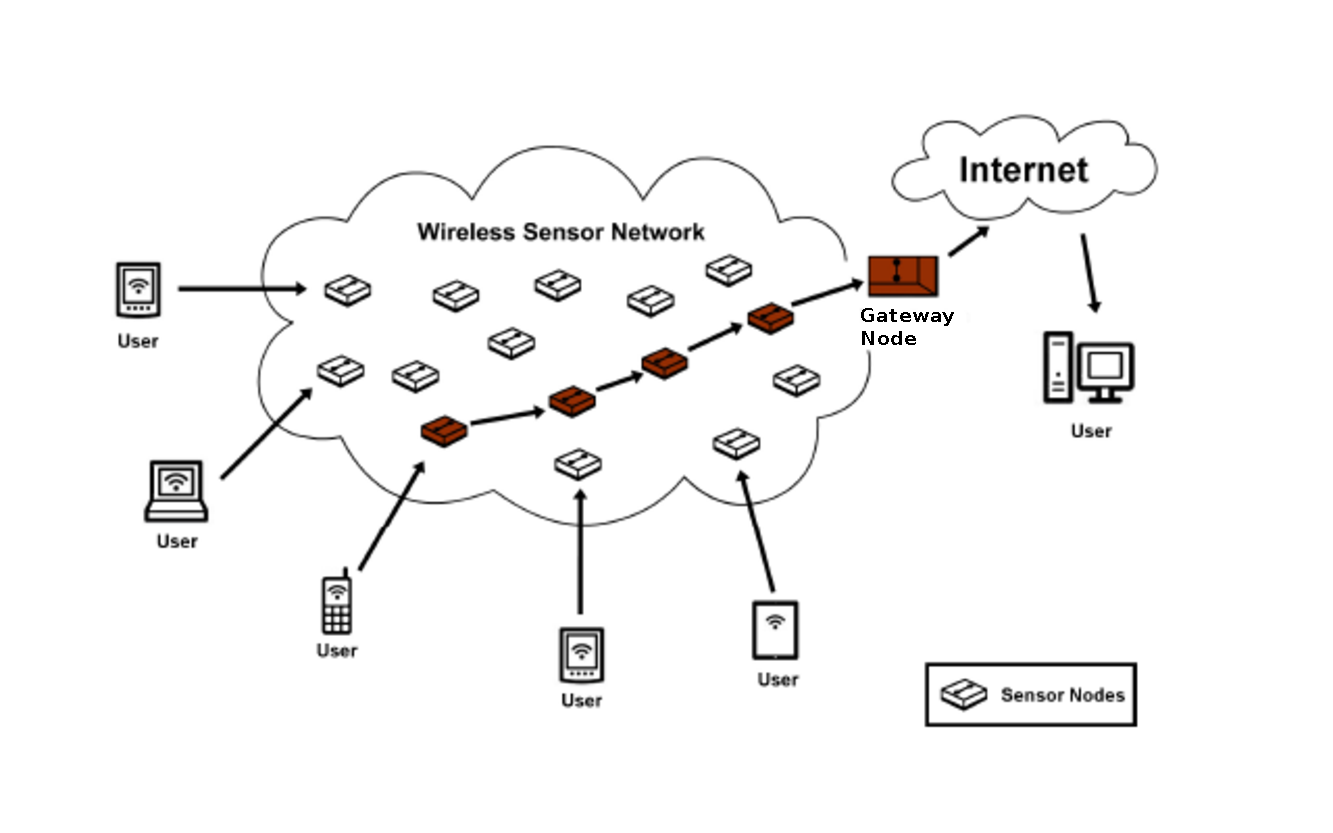
\includegraphics[width=0.8\textwidth]{WSN}
\end{center}
\caption{Overview of Wireless Sensor Networks (WSNs).}
\end{figure}

\section{Applications of WSNs}
Wireless sensor network provides one major advantage over wired
networks: immunity from cabling costs, which gives rise to numerous
applications. Some of them include

\begin{itemize}
\item Disaster handling: Forest Fire Detection, Flood Detection, Earthquake, Detection and surveillance.
\item Military applications: Enemy Tracking, Monitoring Enemy Forces, Biological and Chemical Attacks,
Ammunition detection, Nuclear detection,  Battlefield Surveillance,
etc.
\item Wildlife and Ocean monitoring
\item Manufacturing machinery performance monitoring
\item Structural health Monitoring
\end{itemize}


\section{Security Concerns in WSNs}
As the wireless industry explodes, it faces the growing need for
security. Applications in the sector of economy such as health care,
financial services, and government depend on the underlying security
available for wireless computing environment. Both for authenticated
and private web transactions and signed and encrypted messaging, an
efficient public key infrastructure (PKI) is needed. Privacy assures
that if an eavesdropper is intercepting communication messages are
not. On the other hand, authentication assures that any unauthorized
user cannot fraudulently obtain his/her required services from home
domains \cite{lee2009}. However, the vulnerability of wireless
communication and the ad-hoc nature of deployment open the door for
a wide variety of malicious attacks, making security a key concern
for these applications. Also, the resource constrained nature of
sensor nodes, i.e., limited power, computing and storage resources,
does not allow to use complex security solutions and raises a need
for highly efficient and robust security solutions for WSNs. This
restriction has significantly impacted the field of application
security. Thus, efficient and secure mechanisms for WSNs are
required in order to provide the authenticity and privacy online.
Remote user mutual authentication with key agreement schemes can be
used to achieve some of these security goals and is the major focus
of this thesis.

%\section{Motivation}
\section{Scope and Adopted Approach}
To address the above privacy issues, this thesis proposes an
authentication protocol for WSNs using Elliptic Curve Cryptography
(ECC)-based schemes. The proposed framework is comprised of an
authentication protocol to provide a secure user access to sensor
nodes data. The aim of this research work is to design efficient and
secure authentication protocols to address the authentication
problems in WSNs. The proposed method is discussed in detail in
Chapter \ref{Ch4}.

\section{Thesis Contribution}
The main contributions of the thesis includes
\begin{enumerate}
\item Proposes an user anonymity-preserving authentication scheme with key agreement for WSNs using ECC.
\item Formally analyzes the security of the newly designed protocol as well as its performance.
\item The scheme, as compared to the existing schemes, not only authenticates the users but,
also establishes a session key between the user and the sensor node
after successful mutual authentication.
\item The scheme provides many security and robustness features of user authentication scheme for WSNs.
\end{enumerate}

\section{Roadmap of the Thesis}
The structure of the thesis is as follows:
\begin{enumerate}
\item The Chapter \ref{Ch1} is an introductory part which
discusses the scope of the thesis, about the contribution of this
thesis and the motivation for writing it.

\item The Chapter \ref{Ch2} provides the background of WSNs,
applications of WSNs, security aspects of WSNs, different attacks
existing in WSNs and the user authentication systems in WSNs.

\item The Chapter \ref{Ch3} discusses in details
the basis of ECC, some definitions for security and some
mathematically intractable problems.

\item The Chapter \ref{Ch4} introduces the proposed
authentication framework after highlighting the motivations behind
this work. It also describes the the various phases involved in the
protocol. the protocols have also been pictorially represented.

\item The security analysis comprises of Chapter \ref{Ch5}, where, a formal
security model of the proposed protocol has been discussed. Also the
threat model and trust model used by the proposed framework together
with the assumptions made by it.

\item  The Chapter \ref{Ch6} comprises of the conclusion and further work of the thesis.
\end{enumerate}

\afterpage{\null\newpage}

%%%%%%%%%%%%%%%%%%%%%%%%%%%%%%%%%%%%%%%%%%%%%%%%%%%%%%%%%%%%%%%%%%%%%%%%%%%%%%%%%%%%%%%%%%%%%%%%%%%%%%%%%%%%%%%%%%%%
\chapter{Security in Wireless Sensor Networks}
\label{Ch2} This chapter describes different concepts required for
the understanding of this thesis. This chapter presents an overview
of WSNs security including security objectives, types of attackers
and security attacks in WSNs. It also highlights the constraints in
WSNs which are barriers to provide security.

%\medskip

\section{Characteristics of WSNs}
A WSN can be considered as a special case of ad-hoc networks. A
wireless ad-hoc network does not rely on a fixed infrastructure.
Instead, the nodes in an ad-hoc network organize themselves on the
go to provide pathways for data to be routed from other nodes. They
do not have a fixed topology. The routing decisions in an ad-hoc
network are made dynamically based on the network connectivity. WSNs
share some common features with ad-hoc networks, such as they have
random network topology and infrastructure-less architecture.
Besides, sensor networks possess some characteristics which are
different from ad-hoc networks and traditional wired and wireless
networks. This section reviews the particular characteristics of
a WSN and security concerns in a typical WSN. \\
\linebreak
The following summarizes some of properties of WSNs:

\begin{itemize}
\item \textit{Resource limitation}: Typical sensor nodes are
usually tiny resource constrained devices who have very limited
computational capability, storage capacity, communication bandwidth
and on-board energy available.

\item \textit{Nature of deployment}: In order to achieve the highly
accurate sensing results, the sensor nodes are usually densely
deployed with certain level of redundancy. The number of sensor
nodes in a sensor network may be several orders of magnitude higher
than the nodes in an ad-hoc network.

\item \textit{Dynamic network topology}: The sensor network topology
is unknown prior to the deployment.

\item \textit{Communication}: A sensor node usually has a limited
communication range and every node may not be in direct
communication range of the base station. Therefore, the sensor nodes
send their collected data through intermediate nodes to the nodes
closer to the base station who ultimately forward the data to the
Gateway (GW) node.
\end{itemize}

These characteristics of WSNs offer an advantage to any adversary
($\mathcal{A}$) who intends to compromise  the security. For
instance, the sensor nodes use radio-link as a communication medium
which is in fact insecure. The broadcast nature of communication
medium makes WSNs more vulnerable to security attacks than wired
networks. On the other hand, provision of security in WSNs is a
challenging task since the resources in sensor nodes devices are not
sufficient for executing complex security protocols.

\section{Security Goals}
Security is sometimes seen as a standalone component of a system's
architecture, where security is provided by a separate module.
However, this is usually a flawed approach to the network security.
To achieve a secure system, security must be integrated into every
component, since the components are designed without security can
become a point of attack.\\

\noindent \textit{\textbf{Authentication}} enables each message
sender in the sensor network, including the GW nodes, sensor nodes
and the users, to prove its identity to the receiver, i.e., the
legitimacy of the source of a message. It allows the receiver of the
message to check that received messages are actually originated from
the claimed source.\\

\noindent \textit{\textbf{Message Integrity}} verifies the
genuineness of the received message contents. It must be implemented
to ensure a receiver that the contents of received message have not
been modified in transit by an adversary.\\

\noindent \textit{\textbf{Verification}} empowers each sensor node
in the network to attest the legitimacy of the received message. It
is important to note that authentication does not imply verification
in WSNs environment. A legitimate message sender may send an
authenticated message to the sensor nodes, however, the sensor nodes
may not have access to authentication information of the message
sender or may not be capable of performing efficiently the
computation that is required to verify authentication information.
This capability is ensured by the verification property in WSNs
which enables sensor nodes to verify authenticated messages.
Verification can be seen as a counterpart of authentication where
authentication presents the proof of identity and verification
implies the ability to attest the proof of identity. In WSNs, it is
essential for all three entities to have the ability to confirm that
the message received was actually sent by a trusted sender and not
by an adversary.\\

\noindent \textbf{\textit{Key establishment and Trust setup}} means
when setting up a sensor network, one of the first requirements is
to establish cryptographic keys for later use. Public key
cryptography is another option beyond the capabilities of today's
sensor networks. Its main advantage is that a node can set up a
secure key with any other node in the network.\\

\noindent \textbf{Freshness} means that a received message is new
and a recent one. Freshness could mean both data freshness and key
freshness. Data freshness implies that the received data is recent
and it ensures that no adversary has replayed old messages. Key
freshness implies that the session key established between the two
parties in each session is fresh and it is unique for each
session.\\

\noindent \textit{\textbf{Confidentiality}} prevents unauthorized
parties or adversaries from accessing the data being sent to the
authorized parties. The confidentiality of the message is required
in WSNs to protect the data traveling between the sensor nodes,
between the sensor nodes and the base station, and between the
sensor nodes and the outside users from disclosure. A confidential
message should not reveal its contents to an eavesdropper.\\

\noindent \textbf{\textit{Privacy}} in WSNs is of great concern.
Sensor networks have also thrust privacy concerns to the forefront.
The most obvious risk is that ubiquitous sensor technology might
allow ill-intention individuals to deploy secret surveillance
networks for spying on unaware victims.\\

\noindent \textit{\textbf{Access Control}} ensures that only the
authorized sensor nodes are involved in providing information to
network services and only an authorized user obtains a certain type
of data according to his access privileges. User access control is
required in those applications of WSNs which collect a variety of
data. For such applications, the users have different access
privileges for different types of data due to the data security and
privacy reasons.\\

\noindent \textit{\textbf{Availability}} ensures the survivability
of sensor network services to authorized parties when needed despite
the presence of internal or external attacks.\\

\subsection{Attacks on WSN}
The WSNs are in general a subclass of Wireless networks. So all the
attacks possible on Wireless networks can be directed at WSNs.
However, due to the additional constraints talked about previously,
WSNs gave rise to whole new set of attacks that can be distinguished
into two sets, \textit{"mote-class attacks"} and \textit{"laptop
class attacks"}. The Figure \ref{JJ1} includes different attacks in
WSNs.

\begin{figure}[ht]
\begin{center}
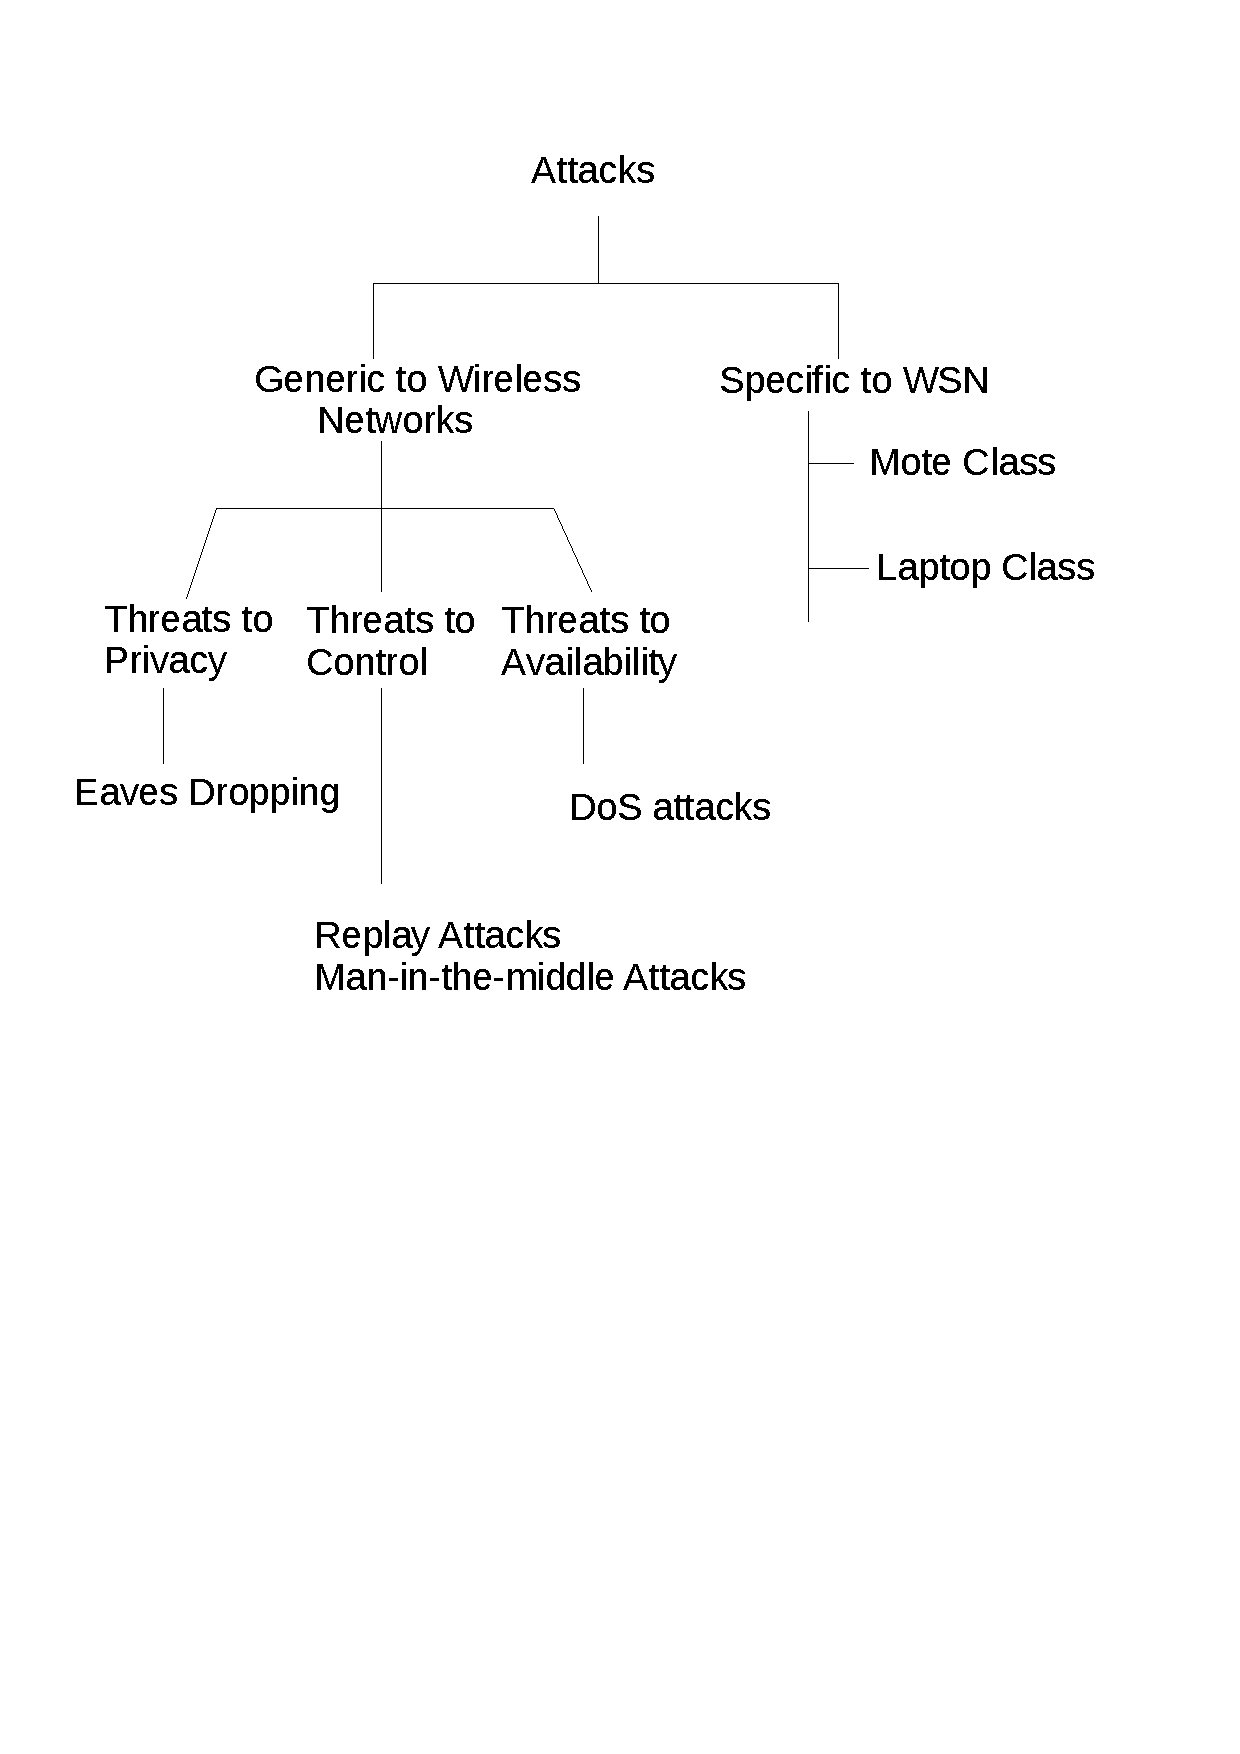
\includegraphics[trim =100 250 100 50, scale=0.5]{./Attacks}
\end{center}
\caption{Figure showing the various attacks possible on WSNs}
\label{JJ1}
\end{figure}


\subsubsection{Threats to Privacy}
\textbf{\textit{Reconnaissance}}: It refers to intelligent gathering
or probing to access the vulnerabilities in a network, to launch a
full-scale attack later. \\

\noindent \textbf{\textit{Eavesdropping}}: It is an operation to
learn the aggregate data that is being collected by the entire network.\\

\subsubsection{Threats to Control}
\noindent\textbf{\textit{Man-in-the-middle attack}}: In this type of
attack, the attacker intrudes into the network and makes an effort
to establish an independent connection between a set of sensor nodes
and the GW node. The nodes in the network are unaware that the
entire flow control is being handled by the attacker. \\

\noindent\textbf{\textit{Replay Attack}}: This is a common attack in
WSN, whereby an attacker is able to intercept user
data and re-transmit user data at a later time.\\

\subsubsection{Threat to Availability}
\noindent\textbf{\textit{Denial of Service(DoS) attack}}: A DoS
attack occurs when an attacker floods the victim with bogus or
spoofed packets with the intent to lower the response rate of the
victim. In the worst-case scenario, it makes the victim
totally unresponsive.\\

\noindent \textbf{\textit{Collision attack}}: Collision attacks
target the MAC layer to create costly exponential back-off. Whenever
collision occurs, the nodes should re-transmit packets affected by
collision, thus, leading to multiple re-transmissions. The amount of
energy expended by the attacker is much less than the energy
expended (battery exhaustion) by the sensor nodes.\\

As attacks on WSNs become more sophisticated, the demand for new
security solutions is continually increasing. Hence, an array of new
security schemes have been designed and implemented in the past
decade \cite{perrig}\cite{healy}. Any security suite must ensure
authentication, integrity, confidentiality, availability, access
control, and non-repudiation. That's why authentication has become
one of the important areas to be taken care when we talk about
wireless protocols.

\section{Authentication}
Authentication is a process by which one verifies that someone is
who he or she claims to be. Authentication enables a receiver of a
message to confirm the

\begin{itemize}
\item claimed message sender or origin of a message (source authentication)
\item contents of a message has not been modified (message integrity).
\end{itemize}

\noindent Based on the types of communication, authentication may be
classified as follows:

\begin{itemize}
\item \textbf{Unicast} or \textbf{Point-to-point} authentication, where the entity authenticates itself to an single entity.
\item \textbf{Multicast} authentication, where the entity authenticates to a small group of entities.
\item \textbf{Broadcast} authentication, where an entity authenticates itself to all entities in the network.
\end{itemize}

\subsection{Authentication in Wireless Sensor Networks}
Beneson \textit{et al.'}s \cite{benenson} talked about the privacy
and distinguished between the insider security and the outsider
security in WSNs as follows:


\begin{itemize}
\item \textit{Insider Security} addresses secure communication in-between the sensors and between the sensors and the GW node(s).
\item \textit{Outsider security} addresses secure communication between the WSN (sensors and GW node) and the outside user.
\end{itemize}
Authentication, which is a part of both insider and outsider
security, is a crucial security requirement in WSNs. In the absence
of a strong authentication mechanism, an adversary can frequently
generate dummy data packets and make the sensor nodes relay them to
deplete their energy. Moreover, a fake or modified message can cause
the sensor nodes to accept wrong information and may result in
serious attacks against the sensor network. For example, it is
important for the GW node to send some crucial information, like the
current time for synchronization, to all sensor nodes in the
network. An adversary can modify a time synchronization message or
send forged data to de-synchronize the network or to disturb the
receiver's clock. A countermeasure to this kind of attacks is
authentication. Authentication in typical WSNs can be classified
into four types:

\begin{itemize}
\item GW node to Sensor node authentication,
\item Sensor node to other sensor node authentication,
\item Sensor Node to User node authentication,
\item GW node to User node authentication.
\end{itemize}

The GW node to sensor nodes authentication has been widely addressed
by the current authentication schemes for WSNs
\cite{perrig,liu,liu2003,drissi,cao}. Sensor Node to other sensor
node authentication has been dealt with by \cite{yasmin}. Sensor
nodes usually collect a variety of data. The data collected by the
sensor nodes is of interest to different types of users such as
research organizations, universities, businesses or individuals. For
example, the humidity level in an area might be a useful piece of
information for a farmer. An individual may be interested to know
about the weather in his surroundings. A researcher may be
interested in environmental data collected by the sensor nodes. An
oil company might be keen to obtain ocean reading data. On the other
hand, the deployment and maintenance cost of a large scale WSNs
makes it difficult for everyone to deploy own sensor networks to
collect data of their interests. The users of the sensor nodes data,
thus take use of these deployment agencies of the large scale WSNs
to obtain this data. Apart from these commercial applications, there
are many army applications which gather sensitive and confidential
data which should be accessible to authorized army officers and
soldiers only. These facts raise the issue of authentication of a
legitimate user in WSNs.\\

Providing a secure user access to sensor nodes data requires two
basic tasks:

\begin{itemize}
\item \textit{User Authentication}: User authentication is a process
by which the system verifies the identity of a user who wants to
access the sensor nodes data. A user authentication mechanism is
necessary to prevent unauthorized users from accessing sensor nodes
data.

\item \textit{Session key establishment}: This enables secure transmission
of confidential sensor nodes data to users after authentication.
\end{itemize}

\subsection{User Authentication}
User authentication in WSNs may be implemented using some user
credentials for instance identity, password, biometric, known only
to the user. It might require sensor nodes to store identity,
password and Biometric triplet of each user. However, a single
compromised node will reveal the passwords and biometric information
of all the users. Alternatively, user authentication may be enforced
with a Public Key Cryptosystem (PKC) with public and private keys. A
simple approach to handle user authentication is a centralized
mechanism. The centralized user authentication schemes described in
\cite{wong,tseng,das,lee2008} divide the user authentication
process into: registration phase, login phase and authentication
phase. In a centralized approach, the user sends his login request
to a central entity, say a GW node. The GW node, after successful
user authentication, forwards the user query to the sensor nodes to
obtain the requested data from them. The GW then replies the user
with data obtained from the sensor nodes. The user can also send the
login request directly to the sensor nodes. The sensor nodes forward
the user information to a central entity e.g., the GW node. The GW
node then verifies the legitimacy of the user request and decides
whether the access should be granted or not. The GW then replies
back to the sensor node with the verification outcomes. Based on the
outcomes, the sensor nodes either provide the requested data to the
user or refuse to process the user request. Both centralized
approaches are simple and easy to deploy because of the fact that
the base station is a powerful device which can perform complex
computations to authenticate a user. An alternative approach to
handle user authentication is a distributed mechanism. In
distributed approach, the sensor nodes who receive the user request
locally verify it and process the user query. There is no
involvement of a third party in this approach \cite{yasmin}.\\


\noindent \textbf{\textit{Limitations:}} Although, the centralized
user authentication schemes are easy to deploy and efficient for
sensor nodes in terms of processing, they all suffer from certain
problems. Firstly, they carry the limitation of a single point of
failure (registration node or GW node). Assume that the third party
authenticates the users and if it fails, then the whole scheme will
fail. Secondly, they require one round trip communication between
the registration node and the sensor node (login node) for every
user request and hence, result in increased communication overhead.
They also cause traffic congestion in the network in case of
multiple simultaneous user requests. Thirdly, they are vulnerable to
a severe DoS attack against sensor network. In this attack, an
adversary sends fake user requests to the login nodes forcing them
to forward fake user requests towards the GW node for verification.
The result is in-network traffic congestion by increased
communication and depletion of sensor nodes battery power while
relaying fake requests. Furthermore, they do not deal with the
session key establishment between the user and the sensor nodes for
secure query and data transfer.

\subsection{Session Key establishment}
To establish a pair-wise key between the user and the sensor nodes,
\cite{jiang} proposes a key establishment scheme based on the
self-certified-PKC \cite{petersen}. In this scheme, the user sends a
request along with his identity to the sensor nodes in his range. In
response to the user request, each sensor node computes a key using
its private key and other public parameters, encrypts a nonce using
the computed key and sends it to the user. The user, if he is the
legitimate one, computes the same key using his own private key and
other public parameters and decrypts the nonce. He then sends the
decrypted nonce back to the sensor node who verifies the correct
decryption. This scheme is efficient in terms of storage and
communication overhead and supports a large number of users as
compared to the other above mentioned user authentication
schemes \cite{yasmin}.\\

\noindent \textit{Limitations:} This scheme only handles the key
establishment between a user and the sensor nodes which implicitly
provides user authentication. The sensor nodes compute a key for
every valid or invalid user request. An adversary may exploit the
situation and launch DoS attack by sending bogus user requests and
forcing sensor nodes to perform the key computations, nonce
encryption and broadcast. The result will be the wastage of sensor
nodes resources. Another issue with this approach is that it always
establishes the same key between a user and a particular sensor node
since there is no involvement of the ephemeral keys. Hence, if a key
established between a user and a particular sensor node has been
compromised once, it will enable the adversary not only to hijack
all future communication between the two participants, but also
decrypt all the previous communication between the same
participants, eavesdropped by the adversary.\\

\afterpage{\null\newpage}
%%%%%%%%%%%%%%%%%%%%%%%%%%%%%%%%%%%%%%%%%%%%%%%%%%%%%%%%%%%%%%%%%%%%%%%%%%%%%%%%%%%%%%%%%%%%%%%%%%%%%%%%%%%%%%%%%%%%%%%%%%%%%%%%

%%%%%%%%%%%%%%%%%%%%%%%%%%%%%%%%%%%%%%%%%%%%%%%%%%%%%%%%%%%%%%%%%%%%%%%%%%%%%%%%%%%%%%%%%%%%%%%%%%%%%%%%%%%%%%%%%%%%%%%%%%%%%%%%
\chapter{Elliptic Curve Cryptography}
\label{Ch3} This chapter reviews the cryptographic tools, primitives
and notions, and describes the computational assumptions used in
this thesis. It also summaries the various formal definitions that
are required to be known for understanding of protocol security.
\medskip
\medskip
\section{Introduction}
Elliptic curves have been studied by mathematicians for a long time.
They have been used to solve a wide range of problems some of them
being the Fermat's Last theorem and Congruent number Problem
\cite{koblitz}. In 1985, Koblitz and Miller independently proposed
using elliptic curves to design PKCs \cite{Lopez}. Since it has been
receiving acceptance throughout the world when standardized
institutions across the world specified elliptic curve protocols.
The algebraic structures of these elliptic curves form the basis of
elliptic curve cryptography (ECC). The fundamental security of this
system relies on the difficulty of solving the discrete logarithm
problem in the elliptic curve group.

\section{Cryptography Basics}
Cryptography involves the design and analysis of mathematical
methods to enable secure communications in the presence of malicious
users (adversaries).

\subsubsection{Basic Model}
In Figure \ref{HH}, entities $A$ (Alice) and $B$ (Bob) are
communicating over an unsecured channel. We assume that all the
communications take place in the presence of an adversary $E$ (Eve)
whose objective is to defeat any security services being provided to
$A$ and $B$.

\begin{figure}
\begin{center}
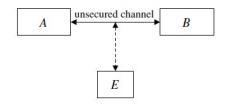
\includegraphics[scale=1.0]{./Basicmodelcomm}
\end{center}
\caption{Basic communications model}\label{HH}
\end{figure}

\subsubsection{Security Goals}
There are few security measures that come into picture while we
design any cryptographic protocol.
\begin{enumerate}
\item \textit{Confidentiality}: It means that keeping data secret from all but those authorized to see it,
messages sent by $A$ to $B$ should not be readable by $E$.

\item \textit{Data origin Authentication}: It means that verifying the source of data, $B$ should be able
to verify that data supposedly sent by $A$ indeed originated with $A$.

\item \textit{Data Integrity}: It ensuring that data has not been altered by unauthorized means, $B$ should
be able to detect when data sent by $A$ has been modified by $E$.

\item \textit{Entity authentication}: It means that verifying the identity of an entity, $B$ should be
convinced of the identity of the other communicating entity.

\item \textit{Non-repudiation}: It means that preventing an entity from denying previous commitments
or actions, when $B$ receives a message purportedly from $A$, not only is $B$ convinced that the
message originated with $A$, but $B$ can convince a neutral third party of this, thus $A$ cannot
deny having sent the message to $B$.
\end{enumerate}

\section{Weierstrass Equation}
Let $p$ be a prime number, and let $\mathbb{F}_q$ denote a finite
field of order $q$ and modulo $p$ (i.e., characteristic is $p$). The
non-singular Weierstrass Equation over $\mathbb{F}_q$ is defined as

\begin{equation}
y^{2} + a_{1}xy + a_{3}y = x^{3} +a_{2}x^{2} +a_{4}x + a_6
\end{equation}
where $a_{1}, a_{2}, a_{3}, a_{4}, a_{6} \in \mathbb{F}_q$. The set
$\mathbb{F}_q$ consists of $(x, y) \in \mathbb{F}_q \times
\mathbb{F}_q$ along with point at infinity($\infty$)
\cite{washington}


\subsection{Elliptic Curve groups}
Let $\mathbb{F}_q$ be an arbitrary field. An elliptic curve $E$ over a field $\mathbb{F}_q$
is a projective non-singular curve defined over $\mathbb{F}_q$ of genus 1 together with a
point $0\in E$ defined over $\mathbb{F}_q$. A Weierstrass equation for an elliptic curve
$E/\mathbb{F}_q$ is an equation of the form:

\begin{equation}
y^{2} = x^{3} + Ax + B
\end{equation}
where $A, \  B \in \mathbb{F}_p$. As the definition of Elliptic
Curve requires it to be non-singular, which means geometrically it
has no cusps, self-intersections or isolated points.Algebraically
the discriminant has been calculated as $\Delta = -16(4A^3 +27B^2)$.
The curve is non-singular if and only if the discriminant is
non-zero or $4A^3 +27B^2 \not\equiv 0 (mod p)$. A pair $(x, y)$,
where $x, y \in \mathbb{F}_q$, is a point on the curve $E$ if $(x,
y)$ satisfies the equation. A example of an elliptic curve has been
shown in Figure \ref{KK}.

\begin{figure}
\begin{center}
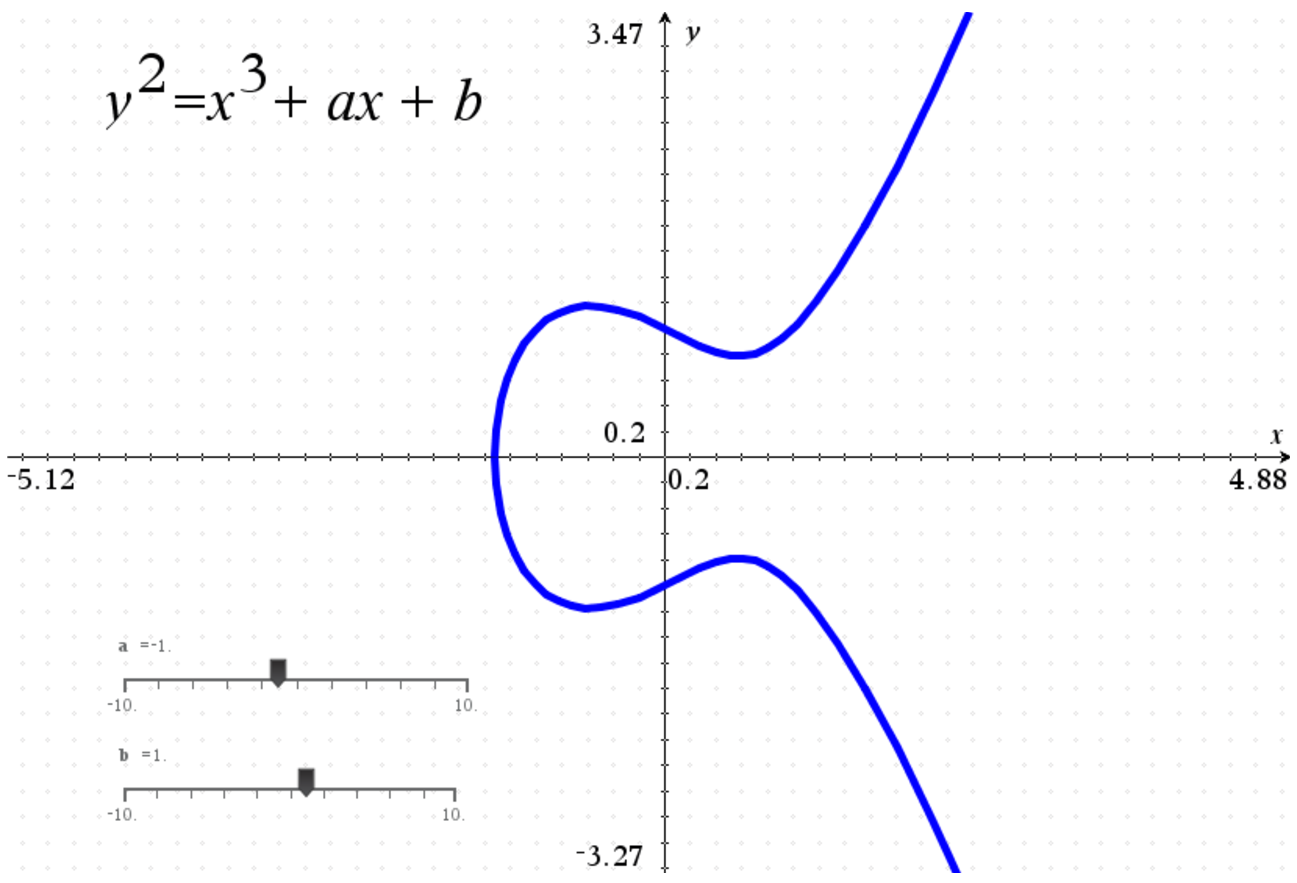
\includegraphics[scale=0.5]{./ec1}
\end{center}
\caption{A Elliptic Curve described by a Weierstrass Equation}
\label{KK}
\end{figure}

\section{Discrete Logarithm}
\begin{definition}
Let $y$ be an arbitrary integer relatively prime to $n$. Let $g$ be
the primitive root of $n$. Let $(G, *)$ be a multiplicative cyclic
group with generator $g$. Let $x$ be an integer randomly selected
from the interval $[1, \phi(n)-1]$ where $\phi(n)$ is the totient
function.

\begin{equation}
y = g^x (mod n)
\end{equation}
The number $x$ is called the discrete logarithm of $y$ with respect to base $g$ modulo $n$.\\
\end{definition}

\begin{corollary}
The \textbf{discrete logarithm problem} in $G$ is defined as the
problem of determining $x$ given $y, g$ and $n$ \cite{patil}.
\end{corollary}

\subsection{Discrete Logarithm Systems}
The first discrete logarithm (DL) system was the key agreement
protocol proposed by Diffie and Hellman in 1976 \cite{diffie}. In
discrete logarithm systems, a key pair is associated with a set of
public domain parameters $(p, q, g)$. Here, $p$ is a prime, $q$ is a
prime divisor of $p-1$, and $g \in [1, p-1]$ has order $q$  ($t = q$
is the smallest positive integer satisfying $g^{t} \equiv 1 (mod
p))$. A private key is an integer x that is selected uniformly at
random from the interval $[1, q -1]$ , and the corresponding public
key is $y = g^{x} \  mod p$. The problem of determining $x$ given
domain parameters $(p, q, g)$ and $y$ is the discrete logarithm
problem (DLP).

\subsection{Elliptic Curve Discrete Log Problem (\textit{ECDLP)}}
Let $E$ be an elliptic curve defined over a finite field
$\mathbb{F}_q$. Let $P$ be a point in $E(\mathbb{F}_{q})$, and
suppose that $P$ has prime order $n$. Then the cyclic subgroup of
$E/\mathbb{F}_q$ generated by $P$ is $\langle P \rangle = \{\infty ,
\ P, \ 2P, \ 3P, \cdots, \ (n-1)P \ \} $. The prime $q$, the
equation of the elliptic curve $E$, and the point $N \in \langle P
\rangle $ and its order $n$, are the public domain parameters.

Let $Q \in \mathbb{F}_q$ of order $q$. A private key is an integer
$d \in \mathbb{Z}$ that is selected uniformly at random from the
interval $[1,n-1]$,  $Q = dN$.

The problem of determining $d$ given the domain parameters and $Q$
is the elliptic curve discrete logarithm problem (ECDLP). The
integer $d$ is called the discrete logarithm of $Q$ base $N$, where
$d= \mbox{log}_{N}Q$.


\section{Diffie-Hellman Problem}
The \textbf{Diffie-Hellman problem (\textit{DHP})} is a mathematical
problem first proposed by Whitfield Diffie and Martin Hellman
\cite{diffie} in the context of cryptography. The problem is stated
as follows.

\begin{definition}
Let $G$ be a cyclic group of order of a large prime $p$ (in practice
it is better to choose the number $p$ such that $(p-1)/2$ is also
prime) generated by an another prime element $g$, and $g$ being the
primitive root of $p$. Given $g$ and the values $g^x$ and $g^y$,
computing the value of $g^{xy}$ is the Diffie-Hellman Problem.
\end{definition}
\subsection{Computational Diffie-Hellman Assumptions}
\begin{definition}
Let $G$ be a finite cyclic group of prime order $p$ generated by
$g$. The CDH assumption states that, given $(g, g^{x}, g^{y})$ for a
randomly chosen generator $g$ and random $x, y \in \{0, 1, 2,
\cdots, p-1\}$, it is computationally intractable to compute the
value $g^{xy}$.
\end{definition}

\subsection{Elliptic Curve Diffie-Hellman Problem (\textit{ECDHP})}
\begin{corollary}
The (computational) Elliptic Curve Diffie-Hellman Problem is stated
as: Given an elliptic curve $E$ defined over a finite field
$\mathbb{F}_q$, a point $P \in E(\mathbb{F}_q)$ of order $n$, and
points $A = aP$, $B = bP \in \langle P \rangle$, calculation of
$abP$ is hard.
\end{corollary}

If ECDLP can be solved on $\langle P \rangle$, then ECDHP can also
be solved efficiently solved by first finding $a$ from $(P, A)$ and
then computing $aB$. Thus, thr ECDHP is no harder than ECDLP to
solve.

\begin{corollary}
The (decisional) Elliptic Curve Diffie-Hellman Problem is stated as:
Given an elliptic curve $E$ defined over a finite field
$\mathbb{F}_q$, a point $P \in E(\mathbb{F}_q)$ of order $n$, and
points $A = aP$, $B = bP \in \langle P \rangle$, the probability
that the adversary ($\mathcal{A}$) succeeds in where the value of
$C$ is $abP$.
\end{corollary}

\begin{remark}
Elliptic Diffie-Hellman key exchange requires Alice and Bob to
exchange points on an elliptic curve. A point Q in $E(\mathbb{F}_p)$
consists of two coordinates $Q = (x_Q, y_Q)$, where $x_Q$ and $y_Q$
are elements of the finite field $\mathbb{F}_p$, so it appears that
Alice must send Bob two numbers in $\mathbb{F}_p$. However, those
two numbers modulo $p$ do not contain as much information as two
arbitrary numbers, since they are related by the formula $y_Q^2 =
x_Q^3 + Ax_Q +B \  \ in  \ \ \mathbb{F}_p$

Note that Eve knows $A$ and $B$, so if she can guess the correct
value of $x_Q$, then there are only two possible values for $y_Q$,
and in practice it is not too hard for her to actually compute the
two values of $y_Q$.

There is thus little reason for Alice to send both coordinates of
$Q_A$ to Bob, since the y-coordinate contains so little additional
information. Instead, she sends Bob only the $x$-coordinate of
$Q_A$. Bob then computes and uses one of the two possible
$y$-coordinates. If he happens to choose the ``correct" $y$, then he
is using $Q_A$, and if he chooses the ``incorrect" $y$ (which is the
negative of the correct $y$), then he is using $Q_A$. In any case,
Bob ends up computing one of $\pm n_B Q_A = \pm (n_A n_B)P$. Then
Alice and Bob use $x$-coordinate as their shared secret value, since
that $x$-coordinate is the same regardless of which $y$ they use.
\end{remark}

\section{Advantages of ECC over others}
The major advantage that Elliptic Curve Cryptography provides is the
reduction in the key size, while providing the same level of security
as RSA \cite{lenstra}. Thus provides faster computations, reduced
power consumption and reduced storage.

\begin{table}[h]
\caption{Table showing key sizes for equivalent security
levels.\cite{eccadv}} \centering \scalebox{.9}{

\begin{tabular}{|| c | c | c ||}
\hline
Symmetric & ECC & DH/DHA/RSA \\[0.5ex]
\hline
80 & 163 & 1024\\
128 & 283 & 3072\\
192 & 409 & 7680\\
256 & 571 & 15,360\\[1ex]
\hline
\end{tabular}}
\end{table}
An elliptic curve over a 163-bit prime field currently gives the
same level of security as 1024-bit RSA modulus or Diffie-Hellman
primes. The difference increases with increase in desired security
levels. 571-bit ECC is currently equivalent to 15,360-bit
RSA/DH/DSA.

This growing difference in key length for equivalent security levels
accounts for performance advantages to be obtained from substituting
RSA with ECC in Public Key Cryptographic protocols.


At 163-bit ECC/1024-bit RSA security level, an elliptic curve
exponentiation for general curves over arbitrary prime fields is
roughly 5 to 15 times faster than RSA operations, depending upon the
platform and optimization. At 256-bit ECC/3072-bit RSA, the ratio
has increased to between 20 to 60 times. For securing 256-bit AES
key, 521-bit ECC is expected to have an advantage of being 400 times
faster than 15,360-bit RSA.

\begin{table}[h]
\caption{Sample Elliptic curve exponentiation and RSA
timings(\textit{in milliseconds}).\cite{eccadv}}
\centering
\scalebox{.9}{
\begin{tabular}{l l l l}
\hline
Processor & MHz & 163-bit ECC & 1024-RSA\\[0.5ex]
\hline
Ultra SPARC II & 450 & 6.1 & 33.8 \\
StrongARM & 200 & 22.9 & 199.5 \\[1ex]
\hline
\end{tabular}}
\end{table}

\afterpage{\null\newpage}




\chapter{Proposed Method}
\label{Ch4} In this chapter, we propose our user authentication
protocol for WSNs. This protocol is a biometric and password based
authenticated key agreement scheme using ECC for wireless sensor
networks. The proposed scheme has four phases: registration phase,
login phase, key-agreement phase and Password Change phase.

\section{Notations}
The following notations are used throughout in the proposed scheme.

%\begin{itemize}
\begin{table}[h]
\caption{Different notations and their meanings}
\centering
\scalebox{.8}{
\begin{tabular}{l   l}
\hline
\textbf{Notations}                   &                                \textbf{Descriptions} \\
\hline
$U$          & User\\
$ID_U$       & Identity of $U$\\
$PW_U$       & Password of $U$\\
$B_U$        & Biometric template of $U$\\
$GW$         & Gateway node of WSN\\
$ID_{GW}$    & Identity of GW\\
$S_{j}$      & Sensor node\\
$s$          & Secret master key of GW node\\
$y$          & Secret known to only GW node sensor node $S_{j}$ \\
$h(\cdot)$   & A secure one-way hash function (e.g., SHA-1)\\
$E_k(\cdot)$ & A symmetric encryption function using AES \cite{AES} with key $k$\\
$d(\cdot)$   & A parametric distance function\\
$\tau$       & A predetermined threshold for biometric verification\\
$F_p$        & A finite field \\
$E$          & An elliptic curve over $F_p$\\
$E(F_{P})$   & Set of all the points on $E$\\
$P$          & Base point of $E(F_{P})$ of order $n$\\
$\oplus$     & Bitwise XOR operation\\
$||$         & Message concatenation operator\\
%\end{itemize}
\hline
\end{tabular}}
\label{F6}
\end{table}

We introduce a new global variable \textit{free} for the GW node,
which is visible to all the other nodes in the network. The variable
\emph{free} is set to 1 (one), if the GW node is free for service
i.e, not busy and GW node accepts the registration or login
requests. After accepting the registration or login requests, the GW
node sets \emph{free} variable to 0 (zero). This factor is takes
care of certain aspects of the DoS attacks. Suppose if the
\textit{free} value is 1 still the GW node is not providing service,
the other nodes can understand that the network has been compromised
by a DOS attacker.

\section{Registration Phase}
Before the user is able to use the sensor node for its purposes for
the first time, it needs to register itself with the GW node of the
network. The following steps are performed.


\begin{figure*}[ht]
\scalebox{0.81}{
\begin{tabular}{|l l l|}
\hline
~~\textbf{User $U$/Smartcard}~~~~~~&                                & ~~~~~~\textbf{GW Node}~~~~~~~~~~~~~~~  \\
\hline
$ID_U$, $PW_U$, $B_U$                             &                                &~~~~~~~~~$(s,y)$                                                   \\
Selects a random number $b_U$ & &\\
$V = h (PW_U || b_U)$ &&\\
$Q = h ((B_U \oplus ID_U))|| b_U)$ &&\\

                                                  & $\underrightarrow{~~~~~~~~~~~~~~~~~~\langle ID_U, V, Q\rangle~~~~~~~~~~~~~~~~~~~~~~}$ & \\
                                                  & ~~~~~~~~~~(via a insecure channel) & \\
&& \\
                               &                       & If $free\neq 1$, reject, else  \\
                               &                       & Update $free = 0$\\
                               &                       & $K_U = h (ID_U || s )$\\
                               &                       & $L_U = h (ID_U || V || Q)$\\
                               &                       & $W_U = h (ID_U \oplus (V || Q)) \oplus K_U$ \\
                               &                       & Generate a random number $n$ \\
                               &                       & $MID = E_{s}(ID_U || n)$ \\
                               &                       & Update $free = 1$\\
                               &&\\
                               & $\underleftarrow{~~\langle\mbox{Smartcard}(ID_{GW}, T_U  ,W_U , MID, h(\cdot)) \rangle~~}$ & \\
                               & ~~~~~~~(via a insecure channel) & \\
&&\\
Store $b_{U}$, $ID_{U}$ &&\\ %%%%%% removed this $Q$...is increasing strage cost by large amount
into the smartcard's memory &&\\
Smart card holds && \\
$\langle ID_{U}, ID_{GW},  b_{U}, L_{U}, W_{U},
MID, h(\cdot)\rangle$ && \\ % Q removed
\hline
\end{tabular}}
\caption{Registration Phase} \label{F4}
\end{figure*}


\begin{enumerate}
\item $U$ inputs his/her identity $ID_{U}$, password $PW_U$ and
biometric $B_U$. $U$ also generates a random number $b_U$ and
computes $V = h(PW_{U} || b_{U})$ and $Q = h((ID_{U} \oplus
B_{U})||b_{U})$. Then $U$ sends $\langle ID_u, V, Q\rangle$ to GW
node in a secure channel.

\item On receiving $\langle ID_u, V, Q\rangle$, if GW is free for receiving request of service, it computes $K_{U}
= h(ID_{U}||s)$. It also computes $L_{U} = h(ID_{U} ||V||Q)$ and $
W_{U} = h(ID_{U} \oplus (V||Q)) \oplus K_U$. The GW node generates a
a random number $n$ and computes $MID = (ID_{U}||n)_{s}$.

\item The GW node then stores $\langle ID_{GW}$, $L_{U}$, $W_{U}$, $MID$,
$h(\cdot)\rangle$ on a new smartcard and sends the smartcard to $U$
over a secure channel, and opens itself up for further requests. On receiving the smartcard, $U$ stores
$b_{U}$, $Q$, $ID_{U}$ on the smartcard. Finally, the smart card
contains the information $\langle ID_{U}$, $ID_{GW}$, , $b_{U}$, %$Q$%
$L_{U}$, $W_{U}$, $MID$, $h(\cdot)\rangle$
\end{enumerate}

\section{Login Phase}

For $U$ to access services and data from the WSN, it needs to login,
performing the following steps:

\begin{enumerate}
\item $U$ inserts his smartcard into the card reader and inputs his
$ID_{U}$, password $PW_{U}$ and personal Biometric $B_{U}^{*}$.

\item The smart card computes $Q^{*} = h((ID_{U}\oplus B_{U}^{*})||b_{U})$
and read $Q$ from the smartcard. If $d(Q^{*},Q) > \tau $, then
rejects the session message. Otherwise, the smart card compute
$V^{*} = h(PW_{U}|| b_{U})$ and hence compute $L_{U}^{*} =
h(ID_{U}||V^{*}||Q^{*})$ and checks if $L_{U}^{*} = L_{U}$. If true
then the smartcard executes the following operations.

\begin{itemize}
\item Compute $K_{U} = W_{U} \oplus h(ID_{U} \oplus (V||Q))$.
\item Generate $\alpha \in F_{P}$.
\item Compute $A = \alpha P$.
\item Choose a current timestamp $T_U$.
\item Compute $M = h(ID_{U}||A||K_{U}||T_{U})$.
\item Send the login message $\langle MID$, $A$, $M$, $T_{U}\rangle$ to $S_{j}$ over a public channel.
\end{itemize}
\end{enumerate}



\begin{figure*}
\begin{center}
\scalebox{.6}{
\begin{tabular}{|l l l|}
\hline
~~~~~~\textbf{User $U$/Smartcard}~~~~~~&      ~~~~~~~~~~~~\textbf{Sensor $S_j$}~~~~~~~~~~~     &~~~~~~~~~~~~~~~~~~~~\textbf{GW-Node}~~~~~~~~\\
\hline
Insert smartcard & &\\
Input $ID_{U}$, $PW_{U}$, $B_U$ & &\\
$Q^* = h ((B_{U}^* \oplus ID_U) || b_U)$ & &\\
%If $d(Q^* , Q) > \tau$ & &\\
%~~~~Reject&&\\
$V*= h( PW_U^{*} || b_U)$ & &\\
$L_U^{*} = h(ID_U^{*} || V^* || Q^* )$ & &\\
If $d(L_U^*, L_U) > \tau$ & &\\
~~~~Reject && \\
$K_U = W_U  \oplus h( ID_U \oplus ( V^{*} || Q^{*}))$ & &\\
Generate $\alpha \in \mathbb{F}_P$ & &\\
$A =  \alpha P$ & &\\
Choose $T_U$ & &\\
$M= h(MID || A ||K_U || T_U)$ & &\\
%$M_1= E_s(MID, M, T_U) $ &&\\
&&\\
$\underrightarrow{~~~~~~~\langle MID,M,  A, T_U \rangle~~~~~~~~}$          & &\\
~~~~~~(via a secure channel) & &\\

                               & Verify $(T_{U}^* - T_U) \leq \Delta T$ &\\
                               & Generate $\beta \in \mathbb{F}_P$ &\\
                               & $B = \beta P$ &\\
                               & Choose $T_S$ &\\
                               & $N = h(y||MID||M||A||B||T_S||ID_S)$ &\\
                               & $M_2= E_y(MID,M,N,T_U,A,B,ID_S)$ &\\
&&\\
                               &$\underrightarrow{~~~~~~~\langle M_2, T_S \rangle~~~~}$    &      \\
                               &~~~(via a secure channel)& \\

                               &                       & If $free\neq 1$, reject \\
                               &                       &~~~~Else \\
                               &                       & Update $free = 0$\\
                               &                       & Decrypt $M_2$ using master key $y$\\
                               &                       & Verify $(T_{S}^* - T_S)\leq \Delta T$\\
                               &                       & Decrypt $MID$ using master key $s$ and get $ID_U$\\
                               &                       & $N^* = h(y||MID||M||A||B||T_S||ID_U)$\\
                               &                       & Verify $N^* = N$\\
                               &                       & $K_U^* = h( ID_U||s)$\\
                               &                       & $M^* = h(MID || A ||K_U^{*}||T_U)$\\
                               &                       & If $M^* \neq M$ \\
                               &                       & ~~~~Reject \\
                               &                       & Generate $n^{\prime}$\\
                               &                       & $MID^{\prime} = E_{s}(ID_U||n^{\prime})$\\
                               &                       & Choose $T_G$\\
                               &                       & $\gamma = h(y||MID^{\prime}||A||T_U||M||ID_S||B||T_S||T_G||ID_{GW})$\\
                               &                       & $\delta = h(ID_U||A||K_U|| T_U ||B||T_S||ID_{GW})$\\
                               &                       & $M_3= E_y(\gamma, h(\delta ), MID^{\prime})$\\
                               &                       & Update $free = 1$\\
&&\\
                               && $\underleftarrow{~~~~~~\langle M_3,T_{G} \rangle~~~~~~}$ \\
                               && ~~~(via a secure channel)  \\
&&\\
                               & Decrypt $M_3$ using master key $y$ &\\
                               & Verify $(T_{G}^* - T_G) \leq \Delta T$ &\\
                               & $\gamma^{*} = h(y||MID^{\prime}||A||T_U||M||ID_S||B||T_S||T_G||ID_{GW})$ &\\
                               & If  $\gamma^{*} \neq \gamma$ &\\
                               & ~~~~Reject &\\
                               & $K = \beta A = \alpha \beta P $ & \\
                               & $sk = h(MID^{\prime}||ID_S||ID_{GW}||A||B||(K\oplus M))$ &\\
                               & $\rho = h(B ||T_S||h(\delta)||sk)$ &\\
                               &&\\
& $\underleftarrow{~~~~~~~\langle MID^{\prime}, B, T_S, T_G, h(\delta), \rho\rangle~~~~~~~~}$  &\\
&~~~(via a secure channel)  &\\

Verify $(T_{S}^* - T_S) \leq \Delta T$ & &\\
Verify $(T_{G}^* - T_G) \leq \Delta T$ & &\\
$K^* = \alpha B = \alpha \beta P $ & &\\
$\delta ^* = h(ID_U||A||K_U|| T_U ||B||T_S||ID_{GW})$ & &\\
If $h(\delta^*) \neq h(\delta)$ & &\\
~~~~Reject&&\\
$sk^* = h(MID^{\prime}||ID_S||ID_{GW}||A||B||(K^{*}\oplus M)$ & &\\
$\rho^{*} = h(B||T_S||h(\delta{*})||sk^{*})$ & & \\
If $\rho^{*} \neq \rho$ & &\\
~~~~Reject && \\
Update $MID$ by $MID^{\prime}$ in smartcard & &\\
\hline
\end{tabular}}
\end{center}
\caption{Login and authentication phase of the proposed scheme}
\label{F5}
\end{figure*}

\section{Key Agreement Phase}
\begin{enumerate}
\item When $S_{j}$ receives the login request at time $T_{U}^{*}$, it
performs the following steps:


\begin{itemize}
\item Check if the flag $free \neq 0$, then reject, otherwise proceed
to next step.
\item Verify if $(T_{U}^{*}-T_{U})<\Delta T$. If it fails the authentication phase is aborted,
where $\Delta T$ is the expected time interval for the transmission
delay of WSN. If on the contrary, it proceeds to the next step.
\item Change the $free$ flag to 0.
\item Generate a random number $\beta \in F_{P}$ and choose a current time stamp $T_{S}$.
\item Compute $B = \beta P$.
\item Compute $N = h(y||MID||A||T_{U}||M||B||T_{S}||ID_{S})$.
\item Send the message $M_2= E_y(MID$, $m$, $T_{U}$, $A$, $B$, $T_{S}$, $ID_{S}$, $N)$, $T_S$ to the GW node over a public channel.
\end{itemize}

\item The GW node then decrypts the $MID$ to get $ID_U$. It computes $N^* = h(y||MID||M||A||B||T_S||ID_U)$ and checks if $N = N^*$. If false then the process stops immediately otherwise,
\begin{itemize}
\item Compute $K_{U} = h(ID_{U}||s)$ and subsequently $M^{*} = h(ID_{U}||A||K_{U}||T_{U})$. Check if $M^{*} = M$, if false, the authentication process is stopped, otherwise,
\item Generate a random number $n^{\prime}$, a time stamp $T_{G}$ and compute $MID^{\prime} = (ID_{U}||n^{\prime})_s$
\item Compute $\gamma = h(y||MID^{\prime}||A||T_U||M||ID_S||B||T_S||T_G||ID_{GW})$ and \\$\delta = h(ID_U||A||K_U|| T_U ||B||T_S||ID_{GW})$
\item Update $free=1$.
\item Send the message $M_3= E_y(\gamma, h(\delta), MID^{\prime}), T_G$ to $S_{j}$ over a public channel.\\
\end{itemize}

\item $S_{j}$ receives ${\gamma, h(\delta), T_G, MID^{\prime}}$ from the GW node, it
needs to verify its origin. It follows the following steps:
\begin{itemize}
 \item Verify if $(T_{G}^{*}-T_{G})<\Delta T$. If it fails the authentication phase is aborted, where $\Delta T$ is the expected time interval for the transmission delay of WSN. If on the contrary, it proceeds to the next step.
 \item Compute  $\gamma^{*} = h(y||MID^{\prime}||A||T_U||M||ID_S||B||T_S||T_G||ID_{GW})$ and verify if  $\gamma ^*= \gamma$. If not then the process is aborted immediately, otherwise, it follows in to the next step.
 \item A key  $K =  \beta A = \alpha \beta P $ is evaluated.
 \item Session key is evaluated as $sk = h(MID^{\prime}||ID_S||ID_{GW}||A||B||(K\oplus M))$.
 \item A mutual authenticator $\rho = h(B ||T_S||h( \delta)||sk)$ is computed an then  it sends $(MID^{\prime}$, $B$, $T_S$, $T_G$, $h(\delta)$, $\rho)$ to $U$.
\end{itemize}

 \item Assume that, $U$ receives the message $(MID^{\prime}$, $B$, $T_S$, $T_G$, $h(\delta)$, $\rho)$ at time $T_{S}^{*}$ and then he doses as follows:
\begin{itemize}
 \item $U$ verifies the two time stamps $T_S$ and $T_G$.
 \item The key $K$ is calculated again, but this time by the user node. Then the mutual authenticator $ \delta $ is computed.
 \item Evaluate $h(\delta ^*) = h(\delta)$. If this is false, the the process is aborted and no session key is established, otherwise it continues to the next step.
 \item The session key $sk$ is computed by the user as $sk^* = h(MID^{\prime}||ID_S||ID_{GW}||A||B||(K^* \oplus M))$.
 \item The second authenticator $\rho$ is computed and crosschecked against the received value from the sensor. If it matches , the user updates the new $MID^{\prime}$ over the old $MID$.
\end{itemize}

\end{enumerate}


\section{Password and Biometric Change Phase}
In this section, we give the password change/update phase. In the
password or biometric change phase , when the user wants to change
his password $PW_U$ to a new password $PW_{U}^{*}$, or his biometric
$B_U$ to $B_{U}^*$, he inserts his smartcard into the terminal and
enters his $ID_U$ and password. The following procedure is followed:

\begin{figure*}[htp]
\centering
\scalebox{1}{
\begin{tabular}{|l l l|}
\hline
~~\textbf{User $U$}~~~~~~&                                 &~~~~~~~~~~~~~~~~~~~~~~~~~~~~~~~~~\textbf{Smartcard}~~~~~~~~~~~~~~~\\
\hline
Enters $ID_U$ and $PW_U$ & &\\
                                                  & & Compute $Q^{*} = h((B_{U} \oplus ID_{U})||b_U)$.\\
                                                  %& & If $d(Q^{*},Q)> \tau$\\
                                                  %& &~~~ Reject\\
                                                  & & Compute $V^{*}=h(PW_{U}^{*} || b_{U})$.\\
                                                  %& & If $V^{*} \neq V$\\
                                                  %& & ~~~ Reject \\
                                                  & & Evaluate $L_U^{*} = h(ID_U^{*} || V^* || Q^* )$ \\
                                                  & & If $d(L_U^*, L_U) > \tau$ \\
                                                  && ~~~~Reject~~~~~ \\
                                                              & & Ask for new password and biometric from $U$ \\
Enters $PW_{U}^{n}$ and $B_{U}^{n}$ & &\\
                                                              & & Compute $Q^{n} =  h((B_{U}^{n} \oplus ID_{U})|| B_{U}^{n})$\\
                                                              & & Compute $V^{n} = h(PW_{U}^{n} ||B_{U}^{n})$\\
                                                              & & Compute  $L_{U}^{n} = h(ID_{U}||V^{n}||Q^{n})$.\\
                                                              & & Compute  $W_{U}^{n}= W_{U} \oplus  h(ID_{U} \oplus (V || Q)) \oplus h(ID_{U} \oplus (V^{n} || Q^{n}))$\\
                          &                                   & Update $L_{U}^{n}$ and $W_{U}^{n}$ in place of $L_U$ and $W_U$ respectively.\\
& & \\
\hline
\end{tabular}}
\caption{Password and Biometric change Phase}
\label{F4}
\end{figure*}
\begin{enumerate}
\item Smartcard validates his $ID_U$ from the data stored in the card.
\item It computes $Q^{*} = h((B_{U} \oplus ID_{U})||b_U)$.
%\item Compare if $d(Q^{*},Q)< \tau$. If false process stops otherwise proceed to the next step.
\item Compute $V^{*} = h(PW_{U}^{*} || b_{U})$.
%\item Compare if $V^{*} = V$. If false process stops otherwise proceed to the next step.
\item Evaluate $L_U^{*} = h(ID_U^{*} || V^* || Q^* )$.
\item Compare if $d(L^{*}, L) < \tau$. If false process stops otherwise proceed to the next step.
\item The user is asked for new password $PW_{U}^{n}$ and Biometric $B_{U}^{n}$.
\item Smartcard computes $Q^{n} =  h((B_{U}^{n} \oplus ID_{U})|| B_{U}^{n})$  and $V^{n} = h(PW_{U}^{n} ||B_{U}^{n})$.
\item Computes $L_{U}^{n} = h(ID_{U}||V^{n}||Q^{n})$.
\item Compute $W_{U}^{n}= W_{U} \oplus  h(ID_{U} \oplus (V || Q)) \oplus h(ID_{U} \oplus (V^{n} || Q^{n}))$
\item Store $L_{U}^{n}$ and $W_{U}^{n}$ in place of $L_U$ and $W_U$ respectively.
\end{enumerate}


\afterpage{\null\newpage}
%%%%%%%%%%%%%%%%%%%%%%%%%%%%%%%%%%%%%%%%%%%%%%%%%%%%%%%%%%%%%%%%%%%%%%%%%%%%%%%%%%%%%%%%%%%%%%%%%%%%%%%
\chapter{Analysis and Comparisons}
\label{Ch5} This chapter presents the formal analysis of the
protocol. We also discuss the various security properties and
compare the performance of our scheme with other related schemes.
\medskip


\section{Security Analysis}
\subsection{Adversary Capabilities}
In this section, we define the semantic security for the session key
and anonymity of user's identity. We define an adversary by
$\mathcal{A}$, and a participant as $P$, where a participant can be
any user or a sensor node.

Assuming there exists $\mathcal{A}$ running in a probabilistic
polynomial time (PPT) in the security parameter $k$, which
represents the bit-length of session keys. We note that the size of
the dictionary $|D|$ is a fixed constant that is independent of the
security parameter $k$. $\mathcal{A}$ has control of all
communications between entities, can request for access to session
keys and long-term keys, and can use side channel analysis to
extract users' information stored on the smart card. These
capabilities of $\mathcal{A}$ are modeled via the following oracle
queries which $\mathcal{A}$ is allowed to make to model the
capabilities .

\begin{itemize}
\item On a hash query $h(q)$ for which there exists a record $(q$, $r)$
appears in $\Lambda_h$, return $r$. Otherwise, choose an element $r
\in\mathbb{Z}_{p}^{*}$, add the record $(q$, $r)$ to the list
$\Lambda_h$ and return $r$.

\item on a query $Send(U$, $start)$, assuming $U$ is in the correct state,
we proceed as described in the protocol and the query is answered by
$(MID$, $M$, $A$, $T_U)$.

\item On a query $Send(S_{i}(MId$, $M$, $A$, $T_U))$, assuming $S_{i}$ is in
correct state, we proceed as described in the protocol and the query
is answered by $(MID$, $M$, $T_U $, $A$, $B$, $T_S$, $ID_S$, $N)$.

\item On a query $Send(G(MID$, $M$, $T_U$, $A$, $B$, $T_S$, $ID_U$, $N))$
assuming $G$ is in the correct state, we proceed as described in the
protocol and the query is answered by $(\gamma$, $h(\delta)$, $T_G$,
$MID^{\prime})$.

\item On a query $Send(S_{i}(\gamma,h(\delta),T_G,MID^{\prime}))$ assuming
$S_{i}$ is in correct state , we proceed as described in the
protocol and the query is answered by $(MID^{\prime}$, $B$,
$h(\delta))$.

\item On a query $Reveal(U_{i})$, we proceed as follows: for an instance
$U$ has accepted, the query is answered with $U$ returning the
session key $sk$.

\item On a query $Execute(U_{i}$, $S_{i}$, $G)$, we proceed using the
simulation of the Send queries and the query is answered with the
transcript $((MID$, $M$, $A$, $T_U)$, $(MID$, $M$, $T_U$, $A$, $B$,
$T_S$, $ID_U$, $N)$, $(\gamma$, $h(\delta)$, $T_G$, $MID^{\prime})$,
$(MID^{\prime}$, $B$, $h(\delta)))$.

\item $CorruptLL(U)$/$CorruptSC(U)$: This query models the corruption
capability of the adversary. The former returns the password of $U$
while the latter returns the information stored in the smart card of
$U$.

\item $CorruptLL(S_i)$: It outputs specific sensor nodes' secret key $y$.

\item $CorruptLL(GW)$: This models the privileged insider attacks.

\item $TestAKE(P)$: This query is used for determining whether the protocol
achieves authenticated key exchange or not. If P has accepted, then
depending on a random bit $b$ chosen by the oracle, $\mathcal{A}$ is
given either the real session key $sk$ if $b = 1$ or a random key
drawn from the session-key space if $b = 0$.

\item $TestAnon(U_{i}$, $ID_{0}$, $ID_{1})$: This query is not used to simulate
the adversary attack, but to define anonymity of user identity.
After querying the oracle, the transcript of $U$'s identity $ID_0$
or $ID_1$ will be returned according to a pre-defined random bit
$c$. If $c=1$ , the adversary will learn the transcript of $U$ with
identity $ID_1$, otherwise with $ID_0$. This query can be called
only once.
\end{itemize}



\subsection{User Anonymity}

The definition of user anonymity is based on the notion of cleanness.

\begin{definition}
(Cleanness) A user $U$ is said to be clean if none of the following occurs:
\begin{enumerate}
\item $\mathcal{A}$ queries both CorruptLL(U) and CorruptSC(U).
\item $\mathcal{A}$ queries CorruptLL(GW)
\end{enumerate}
\end{definition}
User anonymity is formalized  in the context of over the following set of experiments with a few limitations:\\
Experiment \textbf{ExpUA$_0$}:\\
\begin{enumerate}
\item $\mathcal{A}$ is not allowed to make the $TestAnon(U)$ query if the user $U$ is not clean.
\item $\mathcal{A}$ is not allowed to corrupt $GW$ and $U$ if it has already made the $TestAnon(U)$ query.
\item $\mathcal{A}$ is not allowed to access to the $TestAKE(P)$ oracle.
\item $\mathcal{A}$ now outputs a bit $b^{\prime}$ as a guess on the hidden bit $b$
chosen by the $TestUA$ oracle. $\mathcal{A}$ is said to succeed if $b = b^{\prime}$.
\end{enumerate}

Let $SuccUA_0$ be the event that $\mathcal{A}$ succeeds in the
experiment $ExpUA_0$, and $Adv^{UA}_{P}(A)$ denote the advantage of
$\mathcal{A}$ in attacking the user anonymity of protocol $P$. Then,
we define

\begin{equation}
Adv^{UA}_{P}(\mathcal{A}) = 2 \cdot Pr_{P, \mathcal{A}}[SuccUA_0]-1
\label{eq}
\end{equation}

\begin{definition}
(User Anonymity) An authentication and key exchange protocol $P$
provides user anonymity if $Adv^{UA}_P(\mathcal{A})$ is negligible
for any PPT adversary $\mathcal{A}$.
\end{definition}


\begin{theorem}\label{T1}
Our authentication and key exchange protocol, provides user anonymity in the
random oracle model under the \textit{ECDHP} assumption in $G$.
\end{theorem}

\begin{proof}
Let $\mathcal{A}$ be a PPT adversary against the user anonymity
property of protocol. We prove the theorem by making a series of
modifications to the original experiment \textbf{ExpUA$_0$},
bounding the difference in the success probability of \mathcal{A}
between two consecutive experiments, and ending up with an
experiment where \mathcal{A} has a success probability of
$\frac{1}{2}$ (meaning, $\mathcal{A}$ has no advantage). Let
$SuccUA_i$ denote the event that $\mathcal{A}$ correctly guesses the
hidden bit $b$ chosen by the $TestAnon(U)$ oracle in experiment
\textbf{ExpUA$_i$}. Let $t_i^{UA}$ be the maximum time required to
perform the experiment \textbf{ExpUA$_i$} involving $\mathcal{A}$.

\begin{itemize}
\item \textbf{ExpUA$_1$}. In this experiment, we simulate
the random oracle $h$ as follows: For each $h$ query on a string
$s$, the simulator first checks if an entry of the form $(s$, $l)$
is in a list called $HList$ which contains all the input-output
pairs of $h$. If such an entry exists in $HList$, the simulator
returns $l$ as the output of the $h$ query. Otherwise, the simulator
chooses a random $n$-bit string $l^{\prime}$, returns $l^{\prime}$
in response to the query, and adds the entry ($s$, $l^{\prime}$) to
$HList$. For all other oracle queries of $\mathcal{A}$, the
simulator answers them as in the original experiment
\textbf{ExpUA$_0$}. \textbf{ExpUA$_1$} is perfectly
indistinguishable from \textbf{ExpUA$_0$} and therefore, the
following claim is true.

\begin{equation}\label{E1}
Pr_{IA, \mathcal{A}}[SuccUA_1] = Pr_{P, \mathcal{A}}[SuccUA_0]
\end{equation}

\item \textbf{ExpUA$_2$}. Here, we modify the experiment so
that $A$ (the elliptic curve point) is computed as follows:

\begin{enumerate}
\item The simulator chooses a random exponent $x \in \mathbb{Z}_p$ and computes $X = xP$.

\item For each user instance, the simulator chooses a random $\alpha \in \mathbb{Z}_p$ and sets $A = \alpha X$.
As a result of the modification, each $K$ is set to $\alpha x \beta
P$ for some random $\alpha \in \mathbb{Z}_p$. Since the view of $A$
is identical between \textbf{ExpUA$_2$} and \textbf{ExpUA$_1$}, it
follows that:
\end{enumerate}

\begin{equation}\label{E2}
Pr_{IA, \mathcal{A}}[SuccUA_2] = Pr_{P, \mathcal{A}}[SuccUA_1].
\end{equation}

\item \textbf{ExpUA$_3$}. We next modify the computations of $A$ and $B$ as follows:

\begin{enumerate}
\item The simulator chooses two random elements $X, Y \in G$ and sets $B = Y$.

\item For each instance of clean users, the simulator chooses a random
$\alpha \in \mathbb{Z}_p$ and sets $A = \alpha X$. For other
instances, the simulator computes $X$ as in \textbf{ExpUA$_2$}.

\item  For each instance of clean users, the simulator sets each
$sk$ to a random $n$-bit string. For other instances, the simulator
computes $sk$ as in \textbf{ExpUA$_2$}. Since $SK$ is set to a
random $n$-bit string, for clean users, the success probability of
$\mathcal{A}$ may be different between \textbf{ExpUA$_3$} and
\textbf{ExpUA$_2$} if it makes an
H($MID^{\prime}||ID_S||ID_{GW}||A||B||(K \oplus M)$) query. This
difference can be asserted by the claim that

\begin{equation}\label{E3}
|Pr_{P, \mathcal{A}}[SuccUA_3] - Pr_{P, \mathcal{A}}[SuccUA_2]|\leq
1/q_h \cdot Adv^{ECDHP}_G (t^3_UA)
\end{equation}

\noindent where $q_h$ is the number of queries made to the $h$
oracle. The objective of $\mathcal{A}_{ECDHP}$ is to compute and
output the value $W = uvP \in G$ when given an ECDHP-problem
instance ($U = uP$, $V = vP$) $\in G^2$. $\mathcal{A}_{ECDHP}$ runs
$\mathcal{A}$ as a subroutine while simulating all the oracles on
its own.

$\mathcal{A}_{ECDHP}$ handles all the oracle queries of
$\mathcal{A}$ as specified in experiment \textbf{ExpUA$_3$}, but
using $U$ and $V$ in place of $A$ and $B$. When $\mathcal{A}$
outputs its guess $b_0$, $\mathcal{A}_{ECDHP}$ chooses an entry of
the form ($MID^{\prime}||ID_S||ID_{GW}||A||B||(K \oplus M)$) at
random from $HList$ and terminates outputting $K/x \oplus M$. From
the simulation, it is clear that $\mathcal{A}_{ECDHP}$ outputs the
desired result $W = uvP$ with probability at least $1/q_h$ if
$\mathcal{A}$ makes a H($MID^{\prime}||ID_S||ID_{GW}||A||B||(K
\oplus M)$) query for some instance of a clean user $U$. This
completes the proof of this claim.

\item \textbf{ExpUA$_4$}. We finally modify the experiment
so that, for each clean user $U$, a random identity $ID^{\prime}_U$
drawn from the identity space is used in place of the true identity
$ID_U$ in generating $MID$. We see that $\mathcal{A}$ gains no
information on the hidden bit $b$ chosen by the $TestAnon$ oracle
because the identities of all clean users are chosen uniformly at
random from the identity space. It, therefore, follows that $Pr_{IA,
\mathcal{A}}[SuccUA_4] = \frac{1}{2}$.

Thus the last results along with the results \ref{E1}-\ref{E3}, we
get the statement of the Theorem \ref{T1} and also arrive to the
equation \ref{eq}, following which we can choose to check the user
anonymity.
\end{itemize}
\end{proof}


\subsection{Authenticated Key Exchange (AKE) Security}
We need to make sure that our key exchange scheme is resistant to
all kinds of known attacks to authentication protocols. A method of
provable security is used. The security proof is based on a random
oracle model \cite{bellare}.

\begin{theorem}
In the the key agreement phase of the proposed protocol, the mobile user
and the foreign agent correctly generates the same session key between them.
\end{theorem}

\begin{proof}
In Step 3 of key agreement phase, $S_{j}$ generates the session key
as $SK$ $=$ $h(MID^{\prime}$ || $ID_S$ || $ID_{GW}$ || $A$ || $B$ ||
$(K\oplus M))$ and $K$ $=$ $\beta A$ $=$ $\alpha \beta P $. In Step
4, the smartcard of the user generates the session key $SK^*$ $=$
$h(MID^{\prime}$||$ID_U$||$ID_{GW}$||$A$||$B$||$(K^* \oplus M))$ and
$K^*$ $=$ $\alpha B$ $=$ $\alpha \beta P$. Therefore, we have $SK =
SK^*$. Thus, in each session, $U$ and $S_{j}$ always establishes a
fresh and common session key between them.
\end{proof}

\begin{lemma}
\label{Bday}(Birthday Paradox) For a positive integer $N$, and say
$q$ elements $y_1$, $y_2$, $\cdots$, $y_q$  are chosen uniformly and
independently from set of size $N$. The probability that there
exists distinct $i$, $j$ with $y_i$ $=$ $y_j$ is at most
$\frac{q^2}{2N}$.
\end{lemma}

\begin{proof}
Let \textbf{Col} denote an event of collision, i.e there exists $i,
j$ with $y_i = y_j$, and let \textbf{$Col_{i, j}$} denote the event
$y_i = y_j$. Then it is clear that Pr[\textbf{$Col_{i, j}$}]$ = 1/N$
for any distinct $i, j$. Also $Col =  \vee_{i \neq j}Col_{i, j}$ and
so $Pr[Col]$ $=$ $Pr[\vee_{i \neq j}Col_{i, j}] \leq \Sigma_{i \neq
j}Pr[Col_{i, j}]$ $=$ $\frac{q}{2}\cdot\frac{1}{N}$ $\leq
\frac{q^2}{2N}$
\end{proof}

\begin{theorem}
Let $G$ represent group and $D$ uniformly distributed dictionary of
size $|D|$. Let $K$ be our proposed protocol. Let $\mathcal{A}$ be
an adversary against a semantic security within a time bound $t$,
with less than $q_{send}$ Send queries and $q_{exe}$ Execution
queries, and making less than $(q+h)$ random oracle queries. Then we
have
\begin{equation}\label{eq1}

Adv_{K, D}(\mathcal{A}) \leq \frac{2q_{send}}{|D|} + 2q_h
Adv_G^{cdh}(t+(q_{send}+ q_{exe}+1)\tau_{G}) + \frac{2q_{send}}{p}+
\frac{q_h^2 + (q_{send} +q_{exe})^2}{p}
\end{equation}

where $\tau_{G}$ denotes he exponential computation time in $G$
\end{theorem}

\begin{proof}
The proof defines a series of hybrid experiments, starting with a
real attack $Exp_0$ and ending with a experiment $Exp_4$ in which
$\mathcal{A}$ had no advantage. For each experiment $Exp_i$, we
define an even $Succ_i$ depicting the case where the adversary
correctly guess the bit $b$ involved in the \textit{Test-}query. At
the end of the experiments we measure the probability $\Delta_i =
Pr[Succ_{i+1}]- Pr[Succ_{i}]$. Using each difference of the
probability, we get the result of Theorem \ref{T1}.

\begin{itemize}
\item \textbf{Exp\textsubscript{0}}. The experiment corresponds to the
real attack, in the random oracle model model \cite{bellare}. By
definition, we have $Adv_{K, D}(\mathcal{A})= 2Pr[Succ_{0}] -1$. So,

\begin{equation}\label{eq2}
Adv_{K, D}(\mathcal{A})= 2Pr[Succ_{4}] -1 + 2(Pr[Succ_{0} -
Pr[Succ_{4})\leq 2Pr[Succ_4] - 1 + 2 \Sigma_{i = 0}^3 \Delta_i
\end{equation}

\item \textbf{Exp\textsubscript{1}}. In this experiment, we simulate
the random oracles($h$, but also some additional random oracles
$h^{\prime}$ that will appear in $Exp_4$) as usual by maintaining
hash lists $\Lambda_h$ and $\Lambda_{h^{\prime}}$. The
\textit{Execute}, \textit{Reveal}, \textit{Send}, \textit{Corrupt}
and \textit{Test} oracles are also simulated as in the real attack.
One can easily see that this experiment is perfectly
indistinguishable from the real experiment. Hence

\begin{equation}\label{eq3}
\Delta_0 = 0
\end{equation}

\begin{itemize}
\item On a hash query $h(q)$ for which there exists a record $(q$, $r)$
appears in $\Lambda_h$, return $r$. Otherwise choose an element
$r\in\mathbb{Z}_{p}^{*}$, add the record $(q$, $r)$ to the list
$\Lambda_h$ and return $r$.

\item on a query $Send(U, start)$, assuming $U$ is in the correct state,
we proceed as described in the protocol and the query is answered by
$(MID$, $M$, $A$, $T_U)$.

\item On a query $Send(S_{i}(MId$, $M$, $A$, $T_U))$, assuming $S_{i}$
is in correct state, we proceed as described in the protocol and the
query is answered by  $(MID$, $M$, $T_U$, $A$, $B$,$T_S$, $ID_U$,
$N)$.

\item On a query $Send(G(MID$, $M$, $T_U$, $A$, $B$, $T_S$, $ID_U$, $N))$
assuming $G$ is in the correct state, we proceed as described in the
protocol and the query is answered by $(\gamma$, $h(\delta)$, $T_G$,
$MID^{\prime})$.

\item On a query $Send(S_{i}(\gamma$, $h(\delta)$, $T_G$, $MID^{\prime}))$
assuming $S_{i}$ is in correct state , we proceed as described in
the protocol and the query is answered by $(MID^{\prime}$, $B$,
$h(\delta))$

\item On a query $Reveal(U_{i})$, we proceed as follows: for an instance
$U$ has accepted, the query is answered with the session key.

\item On a query $Execute(U_{i}$, $S_{i}$, $G)$, we proceed using the
simulation of the Send queries and the query is answered with the
transcript $((MID$, $M$, $A$, $T_U)$, $(MID$, $M$, $T_U$, $A$, $B$,
$T_S$, $ID_U$, $N)$, $(\gamma$, $h(\delta)$, $T_G$, $MID^{\prime})$,
$(MID^{\prime}$, $B$, $h(\delta)))$

\item On a query $Test(U_{i})$, we proceed as follows, get $SK$ from
$Reveal(U_{i})$ and flip a coin $b$. If $b = 1$, we return the value
of the session key $SK$, otherwise, we return a random value with
the same length.
\end{itemize}

\item \textbf{Exp\textsubscript{2}}. In this experiment, we simulate
all the oracles as in \textbf{Exp\textsubscript{1}}, except that we
halt all executions in which a collision occurs in the transcript
$((MID$, $M$, $A$, $T_U)$, $(MID$, $M$, $T_U$, $A$, $B$, $T_S$,
$ID_U$, $N)$, $(\gamma$, $h(\delta)$, $T_G$, $MID^{\prime})$,
$(MID^{\prime}$, $B$, $h(\delta)))$ . According to the Lemma
\ref{Bday}, the probability of collisions in the output of the $h$
oracle is at most $q^2_{h}/2p$. Similarly, the probability of
collisions in the transcript is at most $(q_{send}+q_{exe})^2/(2p)$,
since $A$, $b_U$ is chosen uniformly at random. Consequently,

\begin{equation}\label{eq4}
\Delta_1 \leq \frac{q_{h}^2+(q_{send}+q_{exe})^2}{2p}
\end{equation}

\item \textbf{Exp\textsubscript{3}}. In this experiment, we abort the
executions wherein $\mathcal{A}$ may have been lucky in guessing the
authentication values $M$, $N$, $\omega$, $\gamma$. The experiments
$Exp_3$ and $Exp_2$ are indistinguishable unless the participants
reject a valid authentication value:

\begin{equation}\label{eq5}
\Delta_2 \leq \frac{q_{send}}{p}.
\end{equation}

\item \textbf{Exp\textsubscript{4}}. In this experiment, we do not
compute the session key using the oracle $h$, but using the private
oracle $h^{\prime}$, so that the values are completely independent
from $A$, $B$. we proceed with the $Execute$ queries $((MID$, $M$,
$A$, $T_U)$, $(MID$, $M$, $T_U$, $A$, $B$, $T_S$, $ID_U$, $N)$,
$(\gamma$, $h(\delta)$, $T_G$, $MID^{\prime})$, $(MID^{\prime}$,
$B$, $h(\delta)))$. The experiments $Exp_3$ and $Exp_4$ are
completely indistinguishable unless the following event
\textbf{AskH} occurs: the adversary $\mathcal{A}$ queries the hash
function $h$. In addition, whatever the bit $b$ involved in the
$Test$ query, the answer is random and independent for all session.
So

\begin{equation}\label{eq6}
\Delta_3 \leq Pr[AskH]
\end{equation}

\begin{equation}\label{eq7}
Pr[Succ_4] = \frac{1}{2}
\end{equation}

To compute the experiment $Exp_4$, we simulate the executions using
the random self-reducabilty of the Elliptic Curve Computational
Diffie-Hellman Problem, given one ECDHP instance $(\alpha P$, $\beta
P)$. We don't need to know the values of $\alpha$ and $\beta$ since
the values of $K$ is not longer needed to compute the session key.
Additionally, for every transcript there only one password which can
be tested by the adversary,so the probability there is
$q_{send}/|D|$. So we can conclude that :

$$Pr[AskH] \leq \frac{q_{send}}{|D|} + q_h Adv_G^{ecdhp}(t+(q_{send}+q_{exe}+1)\cdot \tau_{G})$$
So adding \ref{eq2}-\ref{eq7}, we get the result \ref{eq1}.
\end{itemize}
\end{proof}


\section{Security Properties}
\begin{enumerate}
\item\textbf{Mutual Authentication}
Our scheme provides mutual authentication, where all the entities
are mutually authenticating each other. Like when GW node receives
the message $(MID$, $M$, $T_{U}$, $A$, $B$, $T_{S}$, $ID_{U}$, $N)$
it can make sure that the user message $(MID$, $M$, $T_{U}$, $A)$ is
included in the sensor message to GW node. Similarly the message
$(\gamma$, $h(\delta)$, $T_{G}$, $MID^{\prime})$ when sent by the GW
node to $S_{j}$, the sensor $S_{j}$ sensor can authenticate it and
also further $U$ can authenticate it being from a real GW node and
sensor node.

\item\textbf{Replay Attack}
Our scheme is resistant to replay attack, because the authenticity
of the four messages is validated by checking the timestamps.
Suppose adversary $\mathcal{A}$ intercepts a login message $(MID$,
$M$, $T_{U}$, $A)$ and attempts to access the sensor node by
replaying the same message. The verification fails since the time
difference expires.

\item \textbf{Denial of Service Attacks}
Our scheme is resistant to DoS attacks because the GW node has the
parameter \textit{free} which changes its value once it gets a
request. So if the \textit{free} parameter is 1 and the GW node has
not received any request, the system will detect an intrusion.

\item\textbf{Impersonation Attack}
\begin{itemize}
\item \textit{User:} An attacker can't impersonate the user $U$.
Suppose he forges the login message $(MID, M, T_{U}, A)$. Now he
tries to login into the system with a modified message $(MID, M^{*},
T_{U}, A^{*})$. However, the attacker cant forge $M^{*}$ without
knowing $K$ or the master key $s$ as he will be faced with ECDLP.

\item \textit{Sensor:} As long as the attacker does not possess the
secret key $y$ , he cannot impersonate the sensor and generate $N$.
Similarly, the adversary cannot generate $\rho$, as he does not know
$K$ to generate $\delta$ from that.

\item \textit{GW node:} As long as the attacker does not know $y$,
he cannot generate a valid message for the sensor node.
\end{itemize}

\item \textbf{Stolen Verifier attack}
An attacker who steals the password verifier(like hashed passwords)
from the gateway can use the stolen verifiers to impersonate a legal
user to login into the system. But in our scheme, no such
information is stored at the server , by which the adversary can
make fabricated login request to the server.

\item \textbf{Guessing Attack}(Online/Offline)
Our scheme can resist password guessing attack since in login user
password is not the only thing that is required. It also required
Biometric guessing. An adversary can't guess the $B_U$ from $Q =
h(B_{U} \oplus ID_{U})$ because of one way hash. Similarly guessing
attack on the master key $s$ and $y$ is tough as both are sent as a
digest of secret information.

\item \textbf{Insider Attack}
It may be possible when the GW manager or system administrator can
use user password $PW_{U}$, it impersonate the user $U$ through any
network GW. Our scheme doesn't allow even privileged insiders, as in
registration phase the user passes $V = h(PW_{U}||b_{U})$ instead of
plain $PW_{U}$. here $b_{U}$ is high entropy number not known to GW.
Also in registration phase the smartcard computes $Q = h(ID_{U}
\oplus B_{U})$, so the adversary guessing the correct $B_{U}$ is not
easy because of the one-way hash function. So, this scheme provides
security against insider attacks.

\item \textbf{Redirection Attacks}
When the attacker redirects one's smartcard's communication message
to another one, the sensor node. IN has no information of the
session key $SK$ without mutual authentication and key agreement.
Hence our scheme is safe from redirection attacks.

\item \textbf{Perfect Forward Secrecy}
In our scheme DH key exchange algorithm based on ECC is used to
generate key for session $SK=\alpha\beta P$, perfect forward secrecy
is ensured because an attacker with a compromised all secret key
$(B_{U}, PW_{U}, s, y)$ is only able to obtain $A= \alpha P$ and $B=
\beta P$. Over that computational in-feasibility to obtain session
key $\alpha\beta P$ from $\alpha P$ and $\beta P$ as it is ECDHP
(Elliptic Curve Dille-Helfman Problem). Hence it provides perfect
forward secrecy.

\item \textbf{Known-Session specific temporary information attack (KSSTIA)}
Our Scheme is can resist this kind of attack. We assume that another
adversary $\mathcal{A}$ knows $a$ and $b$. However \textit{A} still
cant know the session key $sk$. We see that $sk$ includes the factor
$K$ which is $\alpha \beta P \oplus M$. So even if the adversary can
calculate $\alpha \beta P$ he can no way know $M$. So cannot compute
random points $\alpha$ and $\beta$ to know $sk$.
\end{enumerate}

\section{Security and Performance Comparisons}
\subsection{Storage Cost}
In our protocol, the only storage that is involved is the smartcard
in the registration phase. To estimate the storage cost, we assume
the following

\begin{enumerate}
\item the size of point in the cyclic group of point $P$ used in the ECC scheme is 320 bits.
\item the block cipher text for AES encryption/decryption is 128 bits.
\item the digest message size of the hash function (SHA-1) is 160 bits.
\item the identity size is 80 bits.
\item and the random number size is 160 bits.
\end{enumerate}

In the registration phase, the GW node computes $L_U$, $W_U$ and
$MID$ and stores them in the smartcard. The size of $L_U$ and $W_U$
are both 160 bits as both of them are digest messages of the hash
function $h(\cdot)$. $MID$ is a symmetric key encryption cipher
text, hence its size is 128 bits. Now when the smartcard reaches the
user, the user appends the random number $b_u$ to the smartcard,
whose size being another 160 bits. So the total cost can be
calculated as to be : $ 160 + 160 +128 + 80 +160 = 688 $ bits.

\begin{table}[h]
\caption{Smartcard storage cost Comparisons of proposed scheme with
other schemes} \centering \scalebox{.9}{
\begin{tabular}{|l c c c c c|}
\hline
                        & Das \cite{das} & Li et al. \cite{li2010efficient} & Das \cite{das2015secure} & Shi\cite{shi} & Proposed  \\
\hline
Smartcard Storage Cost  & 560 bits       & 400 bits                         & 1344 bits                   & 640 bits      & 688 bits \\
\hline
\end{tabular}}
\end{table}


\subsection{Security comparison}
We can recall that protocols of Yuan et al.\cite{yuan}, Yoon et
al.\cite{yoon} do not provide for mutual authentication and can also
be vulnerable to Insider attacks. The security comparisons between
our protocol and some related schemes are summarized in the table
\ref{table:1}.

\begin{table}[h]
\caption{Security Comparisons of proposed scheme with other schemes}
\label{table:1} \centering \scalebox{.75}{
\begin{tabular}{|l llllll|}
 \hline
 Security prop.~~~~~~~~~~~~ & Yuan et al. \cite{yuan} & Das \cite{das} & Yoon et al.\cite{yoon} & Das \cite{das2015secure} & Shi \textit{et al.}'s \cite{shi} & Proposed \\
 [0.5ex]
 \hline
 Stolen verifier Attacks & Secure & Insecure & Secure & Secure & Secure & Secure\\
 Guessing Attacks & Secure & Secure & Secure  & Secure & Secure  & Secure \\
 Impersonation Attacks & Insecure & Insecure & Secure & Secure & Secure & Secure \\
 Replay Attacks & Secure & Secure & Secure & Secure &Secure &  Secure\\
 DoS Attacks & Insecure & Insecure & Insecure &Secure & Insecure & Secure \\
 Insider Attacks & Insecure & Insecure & Secure &Secure& Secure & Secure \\
 Redirection Attacks & Insecure & Insecure & Insecure &Secure& Insecure & Secure \\
 KSSTIA & Insecure & Insecure & Insecure & Insecure & Insecure & Secure \\
 Mutual Authentication & Not Provided & No Provided & Not Provided & Not Provided & Provided & Provided \\
 Perfect Forward Secrecy & Not Provided & Not Provided & Not Provided &Provided & Provided & Provided \\
 Session Key agreement & Not Provided & Not Provided & Not Provided & Provided & Provided & Provided \\
 Message Confidentiality & Not Provided & Provided & Provided & Provided & Provided & Provided \\
 Security Factor & Three-factor & Two-factor & Two-factor & Three-factor & Two-factor & Three-factor \\
 Password Change Phase & Provided & Not Provided & Not Provided & Not Provided & Provided & Provided \\[1ex]
 \hline
\end{tabular}}
\end{table}
\pagebreak
\subsection{Performance Comparison}
We evaluate the performance of the proposed scheme in the terms of the computations and communication costs and compare it with related schemes. To estimate the computation costs, we define the following notations: $t_m$ is the time needed for elliptic curve scalar multiplication, $t_a$ is the time for elliptic curve scalar addition, $t_{enc}$ is the time required for Symmetric key encryption /decryption , $t_h$ is the time for one-way hash function , $t_{grn}$ for generating a random random using a random number generator and $t_{fe} $ is the time for executing fuzzy extractor function(used in Das' Scheme \cite{das2015secure}). The execution time computed by Farash \textit{et al.}'s\cite{farash2013} for the cryptographic operations on different hardware platform is shown in table \ref{table:2}. The execution times have been calculated on an amd64 processor

\begin{table}[h]
\centering
\scalebox{.7}{
\begin{tabular}{|l c c c c c c|}
\hline
Operations & $t_m$ & $t_a$ & $t_{enc}$ & $t_h$ & $t_{grn}$ & $t_{fe}$ \\[0.5ex]
\hline
Execution Time & $0.23 \ ms$ & $1.14  \ ms$ & $ 4.196 \ ms $\cite{paul} & $ 0.001988 \ ms$ & $< 0.0001 \ ms$ & \textbf{PLse give a value, I didnt find} \\[1ex]
\hline
\end{tabular}}
\caption{The execution time of cryptographic operations}
\label{table:2}
\end{table}
To estimate the computational cost , we assume the following
\begin{enumerate}
\item the size of $n$ used in the ECC scheme is 160 bits,
\item the block cipher text for AES encryption/decryption is 128 bits,
\item the digest message size of the hash function (SHA-1) is 160 bits,
\item and the identity size is 80 bits.
\end{enumerate}
To compute the communication cost, we consider all exchanged
messages during a session. In our scheme , the exchanges messages
are $((MID, M,A,T_U),(MID,M,T_U,
A,B,T_S,ID_S,N)$\\,$(\gamma,h(\delta),T_G,MID^{\prime})$,$(MID^{\prime},B,h(\delta)))$.
These message for login phase has a communication cost of 80 bit of
identity, 160 bits of message digest, a block cipher text
containing the $MID$ and an elliptic curve point $P$ of 320 bits. So
the overall cost for the login phase comes out to be $608$ bits. For
the key agreement and mutual authentication phase, we have a
communication cost of $ 3(128) + 5(160) +3(320) + 80 = 2224$ bits.

[\textbf{Yuan Paper for the table below is not available online for free...not able to download for calculating values, also on internet values not available. Pleasse sir, if you have the paper, can you send me.}]

\begin{table}[h]
\begin{center}
\scalebox{.75}{
\begin{tabular}{l c c c c}
\hline
                 &Yuan et al.\cite{yuan}  & AK Das  \cite{das2015secure} & Shi \textit{et al.}'s \cite{shi}& Proposed Protocol\\
\hline
Registration phase && $ 5t_h + 2t_{grn} + t_{fe}$& $4t_h + t_m +t_{grn}$ & $5t_h + 2t_{grn} + t_{enc} $\\
Login phase &&$ 7t_h + t_{grn} + t_{fe}$ & $4t_h + 2t_m + t_{grn}$ & $5t_h +t _m +t_{grn} $\\
Key agreement phase &&$  8t_h + 2t_{enc}$ & $12t_h + 4t_m + t_{grn}$ & $ 12t_h + 3t_m +2t_{grn} + 2t_{enc}$\\
Password Change Phase && Not Provided & $5t_h$ & $ 8t_h$\\

%User computation & & $11t_m + 3t_a + 3t_h \approx 11t_m +3t_a$  & $3t_m +5t_h \approx 3t_m$ & $2t_m + 6 t_h \approx 2t_m$  \\[0.5ex]
%Server Computation &  &$6t_m + 2t_h + 3 t_h \approx 6t_m   $  & $2t_m +3t_h \approx 2t_m $& $2 t_m +4t_h \approx 2t_m$ \\
%GW node computation & & $t_h +t_a \approx t_a$ & $ t_m + 4 t_h \approx t_m$& $4t_h \approx 0$ \\
\hline
\end{tabular}}
\caption{A comparison of  execution times of various phases in various three factor Authentication systems}
\end{center}
\label{table:7}
\end{table}

[\textbf{Sir please I need some some values for the execution times , otherwise I am not able to calculate the correct estimated calculation times for all the protocols. ALso I am searching desparately for three-factor protocols on the internet but I am not able to find anymore. Please sir if you can send me some more, then I will be able to comapre the performances. }]

\begin{table}[h!]
\begin{center}
\scalebox{.75}{
\begin{tabular}{l c c c c}
\hline
Communication Cost                 && Das  \cite{das2015secure} & Shi \textit{et al.}'s \cite{shi}& Proposed Protocol\\
\hline
%Execution time & & $  14.625 ms$& $ 5.16 ms$&$ 3.44 ms$\\
Registration Phase & & $400$ bits & $240$ bits & $400$ bits\\
Login phase & & $400$ bits & $560$ bits & $608$ bits \\
Key Agreement Phase &&$ 528$ bits & $1760$ bits & $1024$ bits\\
Password Change Phase &&$-$&$-$&$-$\\[1ex]
\hline
\end{tabular}}
\caption{The communication costs of cryptographic operations}
\end{center}
\label{table:3}
\end{table}
The performance of the three phases , that is the login phase the
key agreement phase and mutual authentication phase, of the proposed
protocol and a comparison with the related schemes are summarized in
table \ref{table:3}. Although the communication costs of our
protocol is little bit more than Das's Scheme, but as summarised in the table \ref{table:1}, that protocol fails to provide mutual authentication between each node, which is a huge disadvntage as it opens up the possibilty of many masquerading attacks. Our protocol used a 163-bit secure Elliptic Curve Cryptosystem unlike Das's scheme which provided 1024-bit security. Also our protocol
provides better security because of three-factor authentication and
higher efficiency than the rest in terms of execution time,
providing almost speed up by 50\%.






\afterpage{\null\newpage}
\chapter{Conclusion and Further Work}
\label{Ch6} This thesis provides a detailed description of an
Authentication protocol for Wireless Sensor Networks which provides
User Anonymity and Secure Key Exchange and agreement. We also study
the application of Elliptic Curve Cryptography on WSNs. We also
provide a formal analysis of the security of the protocol. We show
that our protocol provides protection against every kind of wireless
sensor attacks known. Also efficiency performance against similar
works have proved to be much better.

\subsubsection{Further Work}
It would be an interesting area of research to look into formal
analysis of authentication protocols. Any formal analysis till date
does not talk about security against various specific attacks. Any
new work proposing such an security proof that takes in account
protection against all the known attacks on WSNs might be a great
future work. Also implementing Functional Encryption in WSNs for
securing message transmissions from Users to Sensors to GW node is a
new path to venture into. Any adversary even if he eavesdrops
messages cannot break the ciphers from the function as he doesn't
have the authority to do so.






\bibliographystyle{acm}
\bibliography{bibliograph}

\end{document}
